\documentclass[11pt,a4paper]{article}

\usepackage[utf8]{inputenc}
\usepackage[T1]{fontenc}
\usepackage[spanish,es-tabla,es-noshorthands]{babel}
\usepackage{lmodern}
\usepackage[a4paper,margin=2.3cm]{geometry}
\usepackage{amsmath,amssymb,mathtools}
\usepackage{bm}
\usepackage{booktabs}
\usepackage{array}
\usepackage{tabularx}
\usepackage{enumitem}
\usepackage[table]{xcolor}
\usepackage{graphicx}
\usepackage[font=small,labelfont=bf]{caption}
\usepackage[most]{tcolorbox}
\usepackage{listings}
\usepackage{tikz}
\usetikzlibrary{arrows.meta,calc,positioning,patterns,decorations.pathmorphing}
\usepackage{microtype}
\usepackage{parskip}
\usepackage{hyperref}

\hypersetup{
  colorlinks=true,
  linkcolor=blue!55!black,
  citecolor=blue!55!black,
  urlcolor=blue!55!black,
  pdftitle={Como resuelve EduFEM el sistema K u = F},
  pdfauthor={EduFEM},
  pdfsubject={Matrices dispersas, factorizacion LU, llenado, minimo grado y SuperLU}
}

% ─── Paleta (la misma de las figuras) ─────────────────────────────────────
\definecolor{serie1}{HTML}{2A78D6}   % azul: EduFEM / NumPy
\definecolor{serie2}{HTML}{EB6834}   % naranja: llenado / SuperLU
\definecolor{serie3}{HTML}{1BAF7A}   % agua: SciPy.sparse
\definecolor{serie4}{HTML}{EDA100}
\definecolor{tinta}{HTML}{0B0B0B}
\definecolor{tinta2}{HTML}{52514E}
\definecolor{tenue}{HTML}{898781}
\definecolor{grilla}{HTML}{E1E0D9}
\definecolor{azulprof}{HTML}{184F95}

% ─── Cajas ────────────────────────────────────────────────────────────────
\tcbuselibrary{skins,breakable}
\newtcolorbox{clave}[1][]{colback=serie1!5,colframe=serie1!75!black,boxrule=0.6pt,arc=2pt,
  left=8pt,right=8pt,top=6pt,bottom=6pt,fonttitle=\bfseries,breakable,#1}
\newtcolorbox{paso}[1][]{colback=gray!3,colframe=tinta2,boxrule=0.5pt,arc=2pt,
  left=7pt,right=7pt,top=5pt,bottom=5pt,fonttitle=\bfseries,breakable,#1}
\newtcolorbox{resultado}[1][]{colback=serie3!6,colframe=serie3!55!black,boxrule=0.6pt,arc=2pt,
  left=8pt,right=8pt,top=6pt,bottom=6pt,fonttitle=\bfseries,breakable,#1}
\newtcolorbox{ojo}[1][]{colback=serie4!9,colframe=serie4!65!black,boxrule=0.5pt,arc=2pt,
  left=7pt,right=7pt,top=5pt,bottom=5pt,fonttitle=\bfseries,breakable,#1}

% ─── Código ───────────────────────────────────────────────────────────────
\lstdefinestyle{py}{
  language=Python, basicstyle=\ttfamily\footnotesize, keywordstyle=\color{azulprof}\bfseries,
  commentstyle=\color{tenue}\itshape, stringstyle=\color{serie2!75!black},
  numbers=left, numberstyle=\tiny\color{tenue}, numbersep=6pt,
  frame=single, rulecolor=\color{grilla}, backgroundcolor=\color{gray!4},
  breaklines=true, showstringspaces=false, columns=fullflexible, keepspaces=true,
  upquote=true, xleftmargin=2em, framexleftmargin=1.6em,
  literate={á}{{\'a}}1 {é}{{\'e}}1 {í}{{\'i}}1 {ó}{{\'o}}1 {ú}{{\'u}}1 {ñ}{{\~n}}1
           {Á}{{\'A}}1 {É}{{\'E}}1 {Í}{{\'I}}1 {Ó}{{\'O}}1 {Ú}{{\'U}}1
           {·}{{$\cdot$}}1 {—}{{---}}1 {→}{{$\to$}}1 {ν}{{$\nu$}}1
}
\lstdefinestyle{algo}{basicstyle=\ttfamily\small, columns=fullflexible, keepspaces=true,
  frame=single, rulecolor=\color{grilla}, backgroundcolor=\color{gray!4}, xleftmargin=0.5em,
  framexleftmargin=0.3em, mathescape=true,
  literate={ℓ}{{$\ell$}}1 {≠}{{$\neq$}}1 {←}{{$\leftarrow$}}1 {−}{{$-$}}1 {π}{{$\pi$}}1
           {·}{{$\cdot$}}1 {á}{{\'a}}1 {é}{{\'e}}1 {í}{{\'i}}1 {ó}{{\'o}}1 {ú}{{\'u}}1 {ñ}{{\~n}}1}

% ─── TikZ ─────────────────────────────────────────────────────────────────
\tikzset{
  nodo/.style={circle,draw=tinta2,fill=white,line width=0.6pt,inner sep=0pt,minimum size=5mm,font=\scriptsize},
  nodoelim/.style={circle,draw=tenue!70,dashed,fill=white,inner sep=0pt,minimum size=5mm,font=\scriptsize,text=tenue!90},
  nodosig/.style={circle,draw=serie1,fill=serie1,text=white,line width=0.6pt,inner sep=0pt,minimum size=5mm,font=\scriptsize\bfseries},
  arista/.style={draw=tinta2!75,line width=0.55pt},
  relleno/.style={draw=serie2,line width=1.2pt,dash pattern=on 2.6pt off 1.4pt},
  grado/.style={font=\tiny\bfseries,text=azulprof,fill=white,inner sep=0.5pt,rounded corners=1pt},
  resorte/.style={decorate,decoration={zigzag,segment length=5pt,amplitude=3pt,pre length=5pt,post length=5pt},line width=0.7pt,draw=tinta2},
}

% ─── Cifras medidas (las escribe generar_datos.py) ────────────────────────
\newcommand{\cifra}[1]{\ifcsname cifra:#1\endcsname\csname cifra:#1\endcsname\else
  \textbf{\textcolor{red}{??}}\PackageWarning{cifras}{Falta la cifra #1}\fi}
% Generado por generar_datos.py: no editar a mano.
\expandafter\def\csname cifra:scipy\endcsname{1.17.1}
\expandafter\def\csname cifra:numpy\endcsname{2.4.6}
\expandafter\def\csname cifra:python\endcsname{3.13.9}
\expandafter\def\csname cifra:fecha\endcsname{2026-09-23}
\expandafter\def\csname cifra:permc\endcsname{MMD\_AT\_PLUS\_A}
\expandafter\def\csname cifra:q9:8:nodos\endcsname{289}
\expandafter\def\csname cifra:q9:8:elementos\endcsname{64}
\expandafter\def\csname cifra:q9:8:gdl\endcsname{578}
\expandafter\def\csname cifra:q9:8:restr\endcsname{34}
\expandafter\def\csname cifra:q9:8:n\endcsname{544}
\expandafter\def\csname cifra:q9:8:tripletes\endcsname{20\,736}
\expandafter\def\csname cifra:q9:8:nnzK\endcsname{16\,900}
\expandafter\def\csname cifra:q9:8:nnzKr\endcsname{15\,600}
\expandafter\def\csname cifra:q9:8:maxfila\endcsname{50}
\expandafter\def\csname cifra:q9:8:nnzAtA\endcsname{54\,208}
\expandafter\def\csname cifra:q9:8:maxfilaAtA\endcsname{162}
\expandafter\def\csname cifra:q9:8:duplicados\endcsname{3836}
\expandafter\def\csname cifra:q9:8:densK\endcsname{5{,}06}
\expandafter\def\csname cifra:q9:8:densKr\endcsname{5{,}27}
\expandafter\def\csname cifra:q9:8:razonAtA\endcsname{3{,}5}
\expandafter\def\csname cifra:q9:8:mbKr\endcsname{0{,}19}
\expandafter\def\csname cifra:q9:8:mbDenso\endcsname{2{,}4}
\expandafter\def\csname cifra:q9:8:gbInv\endcsname{0{,}0}
\expandafter\def\csname cifra:q9:8:lu:NATURAL\endcsname{232\,880}
\expandafter\def\csname cifra:q9:8:rel:NATURAL\endcsname{14{,}9}
\expandafter\def\csname cifra:q9:8:t:NATURAL\endcsname{0{,}019}
\expandafter\def\csname cifra:q9:8:ms:NATURAL\endcsname{19}
\expandafter\def\csname cifra:q9:8:piv:NATURAL\endcsname{36}
\expandafter\def\csname cifra:q9:8:flops:NATURAL\endcsname{\ensuremath{6{,}5\times 10^{7}}}
\expandafter\def\csname cifra:q9:8:lu:COLAMD\endcsname{39\,952}
\expandafter\def\csname cifra:q9:8:rel:COLAMD\endcsname{2{,}6}
\expandafter\def\csname cifra:q9:8:t:COLAMD\endcsname{0{,}0025}
\expandafter\def\csname cifra:q9:8:ms:COLAMD\endcsname{2{,}5}
\expandafter\def\csname cifra:q9:8:piv:COLAMD\endcsname{54}
\expandafter\def\csname cifra:q9:8:flops:COLAMD\endcsname{\ensuremath{1{,}5\times 10^{6}}}
\expandafter\def\csname cifra:q9:8:lu:MMD_ATA\endcsname{40\,740}
\expandafter\def\csname cifra:q9:8:rel:MMD_ATA\endcsname{2{,}6}
\expandafter\def\csname cifra:q9:8:t:MMD_ATA\endcsname{0{,}0041}
\expandafter\def\csname cifra:q9:8:ms:MMD_ATA\endcsname{4{,}1}
\expandafter\def\csname cifra:q9:8:piv:MMD_ATA\endcsname{32}
\expandafter\def\csname cifra:q9:8:flops:MMD_ATA\endcsname{\ensuremath{1{,}9\times 10^{6}}}
\expandafter\def\csname cifra:q9:8:lu:MMD_AT_PLUS_A\endcsname{27\,104}
\expandafter\def\csname cifra:q9:8:rel:MMD_AT_PLUS_A\endcsname{1{,}7}
\expandafter\def\csname cifra:q9:8:t:MMD_AT_PLUS_A\endcsname{0{,}0020}
\expandafter\def\csname cifra:q9:8:ms:MMD_AT_PLUS_A\endcsname{2{,}0}
\expandafter\def\csname cifra:q9:8:piv:MMD_AT_PLUS_A\endcsname{10}
\expandafter\def\csname cifra:q9:8:flops:MMD_AT_PLUS_A\endcsname{\ensuremath{7{,}9\times 10^{5}}}
\expandafter\def\csname cifra:q9:8:flopsDensa\endcsname{\ensuremath{1{,}1\times 10^{8}}}
\expandafter\def\csname cifra:q9:8:flopsInv\endcsname{\ensuremath{3{,}2\times 10^{8}}}
\expandafter\def\csname cifra:q9:8:gflops\endcsname{0{,}39}
\expandafter\def\csname cifra:q9:8:xflopsDensa\endcsname{140}
\expandafter\def\csname cifra:q9:8:xflops:NATURAL\endcsname{82{,}9}
\expandafter\def\csname cifra:q9:8:xflops:COLAMD\endcsname{2{,}0}
\expandafter\def\csname cifra:q9:8:xflops:MMD_ATA\endcsname{2{,}5}
\expandafter\def\csname cifra:q9:8:mbLU\endcsname{0{,}33}
\expandafter\def\csname cifra:q9:8:nnzL\endcsname{13\,824}
\expandafter\def\csname cifra:q9:8:nnzU\endcsname{13\,824}
\expandafter\def\csname cifra:q9:8:LigualU\endcsname{sí}
\expandafter\def\csname cifra:q9:8:sn:media\endcsname{4{,}3}
\expandafter\def\csname cifra:q9:8:sn:max\endcsname{52}
\expandafter\def\csname cifra:q9:8:sn:mayor1\endcsname{100}
\expandafter\def\csname cifra:q9:8:lu0\endcsname{27\,104}
\expandafter\def\csname cifra:q9:8:piv0\endcsname{0}
\expandafter\def\csname cifra:q9:8:pivpct\endcsname{1{,}8}
\expandafter\def\csname cifra:q9:8:x:NATURAL\endcsname{9{,}4}
\expandafter\def\csname cifra:q9:8:xlu:NATURAL\endcsname{8{,}6}
\expandafter\def\csname cifra:q9:8:x:COLAMD\endcsname{1{,}3}
\expandafter\def\csname cifra:q9:8:xlu:COLAMD\endcsname{1{,}5}
\expandafter\def\csname cifra:q9:8:x:MMD_ATA\endcsname{2{,}0}
\expandafter\def\csname cifra:q9:8:xlu:MMD_ATA\endcsname{1{,}5}
\expandafter\def\csname cifra:q9:8:tsolve\endcsname{0{,}0092}
\expandafter\def\csname cifra:q9:8:tinv\endcsname{0{,}027}
\expandafter\def\csname cifra:q9:8:xsolve\endcsname{5}
\expandafter\def\csname cifra:q9:8:xinv\endcsname{14}
\expandafter\def\csname cifra:q9:8:xinvsolve\endcsname{3{,}0}
\expandafter\def\csname cifra:q9:8:res:sp\endcsname{\ensuremath{1{,}1\times 10^{-12}}}
\expandafter\def\csname cifra:q9:8:res:solve\endcsname{\ensuremath{1{,}6\times 10^{-12}}}
\expandafter\def\csname cifra:q9:8:res:inv\endcsname{\ensuremath{1{,}3\times 10^{-12}}}
\expandafter\def\csname cifra:q9:8:difinv\endcsname{\ensuremath{5{,}3\times 10^{-13}}}
\expandafter\def\csname cifra:q9:8:densInv\endcsname{100}
\expandafter\def\csname cifra:q9:8:cerosInv\endcsname{0}
\expandafter\def\csname cifra:q9:8:cond\endcsname{\ensuremath{5{,}8\times 10^{4}}}
\expandafter\def\csname cifra:q9:16:nodos\endcsname{1089}
\expandafter\def\csname cifra:q9:16:elementos\endcsname{256}
\expandafter\def\csname cifra:q9:16:gdl\endcsname{2178}
\expandafter\def\csname cifra:q9:16:restr\endcsname{66}
\expandafter\def\csname cifra:q9:16:n\endcsname{2112}
\expandafter\def\csname cifra:q9:16:tripletes\endcsname{82\,944}
\expandafter\def\csname cifra:q9:16:nnzK\endcsname{66\,564}
\expandafter\def\csname cifra:q9:16:nnzKr\endcsname{63\,984}
\expandafter\def\csname cifra:q9:16:maxfila\endcsname{50}
\expandafter\def\csname cifra:q9:16:nnzAtA\endcsname{239\,040}
\expandafter\def\csname cifra:q9:16:maxfilaAtA\endcsname{162}
\expandafter\def\csname cifra:q9:16:duplicados\endcsname{16\,380}
\expandafter\def\csname cifra:q9:16:densK\endcsname{1{,}40}
\expandafter\def\csname cifra:q9:16:densKr\endcsname{1{,}43}
\expandafter\def\csname cifra:q9:16:razonAtA\endcsname{3{,}7}
\expandafter\def\csname cifra:q9:16:mbKr\endcsname{0{,}78}
\expandafter\def\csname cifra:q9:16:mbDenso\endcsname{36}
\expandafter\def\csname cifra:q9:16:gbInv\endcsname{0{,}0}
\expandafter\def\csname cifra:q9:16:lu:NATURAL\endcsname{3\,422\,064}
\expandafter\def\csname cifra:q9:16:rel:NATURAL\endcsname{53{,}5}
\expandafter\def\csname cifra:q9:16:t:NATURAL\endcsname{1{,}7}
\expandafter\def\csname cifra:q9:16:ms:NATURAL\endcsname{1700}
\expandafter\def\csname cifra:q9:16:piv:NATURAL\endcsname{74}
\expandafter\def\csname cifra:q9:16:flops:NATURAL\endcsname{\ensuremath{3{,}7\times 10^{9}}}
\expandafter\def\csname cifra:q9:16:lu:COLAMD\endcsname{288\,656}
\expandafter\def\csname cifra:q9:16:rel:COLAMD\endcsname{4{,}5}
\expandafter\def\csname cifra:q9:16:t:COLAMD\endcsname{0{,}018}
\expandafter\def\csname cifra:q9:16:ms:COLAMD\endcsname{18}
\expandafter\def\csname cifra:q9:16:piv:COLAMD\endcsname{117}
\expandafter\def\csname cifra:q9:16:flops:COLAMD\endcsname{\ensuremath{2{,}0\times 10^{7}}}
\expandafter\def\csname cifra:q9:16:lu:MMD_ATA\endcsname{271\,868}
\expandafter\def\csname cifra:q9:16:rel:MMD_ATA\endcsname{4{,}2}
\expandafter\def\csname cifra:q9:16:t:MMD_ATA\endcsname{0{,}029}
\expandafter\def\csname cifra:q9:16:ms:MMD_ATA\endcsname{29}
\expandafter\def\csname cifra:q9:16:piv:MMD_ATA\endcsname{48}
\expandafter\def\csname cifra:q9:16:flops:MMD_ATA\endcsname{\ensuremath{2{,}5\times 10^{7}}}
\expandafter\def\csname cifra:q9:16:lu:MMD_AT_PLUS_A\endcsname{156\,040}
\expandafter\def\csname cifra:q9:16:rel:MMD_AT_PLUS_A\endcsname{2{,}4}
\expandafter\def\csname cifra:q9:16:t:MMD_AT_PLUS_A\endcsname{0{,}013}
\expandafter\def\csname cifra:q9:16:ms:MMD_AT_PLUS_A\endcsname{13}
\expandafter\def\csname cifra:q9:16:piv:MMD_AT_PLUS_A\endcsname{18}
\expandafter\def\csname cifra:q9:16:flops:MMD_AT_PLUS_A\endcsname{\ensuremath{8{,}0\times 10^{6}}}
\expandafter\def\csname cifra:q9:16:flopsDensa\endcsname{\ensuremath{6{,}3\times 10^{9}}}
\expandafter\def\csname cifra:q9:16:flopsInv\endcsname{\ensuremath{1{,}9\times 10^{10}}}
\expandafter\def\csname cifra:q9:16:gflops\endcsname{0{,}62}
\expandafter\def\csname cifra:q9:16:xflopsDensa\endcsname{780}
\expandafter\def\csname cifra:q9:16:xflops:NATURAL\endcsname{457}
\expandafter\def\csname cifra:q9:16:xflops:COLAMD\endcsname{2{,}6}
\expandafter\def\csname cifra:q9:16:xflops:MMD_ATA\endcsname{3{,}1}
\expandafter\def\csname cifra:q9:16:mbLU\endcsname{1{,}9}
\expandafter\def\csname cifra:q9:16:nnzL\endcsname{79\,076}
\expandafter\def\csname cifra:q9:16:nnzU\endcsname{79\,076}
\expandafter\def\csname cifra:q9:16:LigualU\endcsname{sí}
\expandafter\def\csname cifra:q9:16:sn:media\endcsname{4{,}1}
\expandafter\def\csname cifra:q9:16:sn:max\endcsname{110}
\expandafter\def\csname cifra:q9:16:sn:mayor1\endcsname{100}
\expandafter\def\csname cifra:q9:16:lu0\endcsname{156\,040}
\expandafter\def\csname cifra:q9:16:piv0\endcsname{0}
\expandafter\def\csname cifra:q9:16:pivpct\endcsname{0{,}9}
\expandafter\def\csname cifra:q9:16:x:NATURAL\endcsname{133}
\expandafter\def\csname cifra:q9:16:xlu:NATURAL\endcsname{21{,}9}
\expandafter\def\csname cifra:q9:16:x:COLAMD\endcsname{1{,}4}
\expandafter\def\csname cifra:q9:16:xlu:COLAMD\endcsname{1{,}8}
\expandafter\def\csname cifra:q9:16:x:MMD_ATA\endcsname{2{,}2}
\expandafter\def\csname cifra:q9:16:xlu:MMD_ATA\endcsname{1{,}7}
\expandafter\def\csname cifra:q9:16:tsolve\endcsname{0{,}85}
\expandafter\def\csname cifra:q9:16:tinv\endcsname{1{,}7}
\expandafter\def\csname cifra:q9:16:xsolve\endcsname{66}
\expandafter\def\csname cifra:q9:16:xinv\endcsname{135}
\expandafter\def\csname cifra:q9:16:xinvsolve\endcsname{2{,}0}
\expandafter\def\csname cifra:q9:16:res:sp\endcsname{\ensuremath{3{,}0\times 10^{-12}}}
\expandafter\def\csname cifra:q9:16:res:solve\endcsname{\ensuremath{7{,}5\times 10^{-12}}}
\expandafter\def\csname cifra:q9:16:res:inv\endcsname{\ensuremath{3{,}9\times 10^{-12}}}
\expandafter\def\csname cifra:q9:16:difinv\endcsname{\ensuremath{2{,}1\times 10^{-13}}}
\expandafter\def\csname cifra:q9:16:densInv\endcsname{100}
\expandafter\def\csname cifra:q9:16:cerosInv\endcsname{0}
\expandafter\def\csname cifra:q9:16:cond\endcsname{\ensuremath{2{,}3\times 10^{5}}}
\expandafter\def\csname cifra:q9:24:nodos\endcsname{2401}
\expandafter\def\csname cifra:q9:24:elementos\endcsname{576}
\expandafter\def\csname cifra:q9:24:gdl\endcsname{4802}
\expandafter\def\csname cifra:q9:24:restr\endcsname{98}
\expandafter\def\csname cifra:q9:24:n\endcsname{4704}
\expandafter\def\csname cifra:q9:24:tripletes\endcsname{186\,624}
\expandafter\def\csname cifra:q9:24:nnzK\endcsname{148\,996}
\expandafter\def\csname cifra:q9:24:nnzKr\endcsname{145\,136}
\expandafter\def\csname cifra:q9:24:maxfila\endcsname{50}
\expandafter\def\csname cifra:q9:24:nnzAtA\endcsname{554\,944}
\expandafter\def\csname cifra:q9:24:maxfilaAtA\endcsname{162}
\expandafter\def\csname cifra:q9:24:duplicados\endcsname{37\,628}
\expandafter\def\csname cifra:q9:24:densK\endcsname{0{,}65}
\expandafter\def\csname cifra:q9:24:densKr\endcsname{0{,}66}
\expandafter\def\csname cifra:q9:24:razonAtA\endcsname{3{,}8}
\expandafter\def\csname cifra:q9:24:mbKr\endcsname{1{,}8}
\expandafter\def\csname cifra:q9:24:mbDenso\endcsname{180}
\expandafter\def\csname cifra:q9:24:gbInv\endcsname{0{,}2}
\expandafter\def\csname cifra:q9:24:lu:NATURAL\endcsname{16\,842\,032}
\expandafter\def\csname cifra:q9:24:rel:NATURAL\endcsname{116{,}0}
\expandafter\def\csname cifra:q9:24:t:NATURAL\endcsname{13}
\expandafter\def\csname cifra:q9:24:ms:NATURAL\endcsname{13\,000}
\expandafter\def\csname cifra:q9:24:piv:NATURAL\endcsname{115}
\expandafter\def\csname cifra:q9:24:flops:NATURAL\endcsname{\ensuremath{4{,}0\times 10^{10}}}
\expandafter\def\csname cifra:q9:24:lu:COLAMD\endcsname{928\,768}
\expandafter\def\csname cifra:q9:24:rel:COLAMD\endcsname{6{,}4}
\expandafter\def\csname cifra:q9:24:t:COLAMD\endcsname{0{,}075}
\expandafter\def\csname cifra:q9:24:ms:COLAMD\endcsname{75}
\expandafter\def\csname cifra:q9:24:piv:COLAMD\endcsname{219}
\expandafter\def\csname cifra:q9:24:flops:COLAMD\endcsname{\ensuremath{1{,}0\times 10^{8}}}
\expandafter\def\csname cifra:q9:24:lu:MMD_ATA\endcsname{805\,480}
\expandafter\def\csname cifra:q9:24:rel:MMD_ATA\endcsname{5{,}5}
\expandafter\def\csname cifra:q9:24:t:MMD_ATA\endcsname{0{,}078}
\expandafter\def\csname cifra:q9:24:ms:MMD_ATA\endcsname{78}
\expandafter\def\csname cifra:q9:24:piv:MMD_ATA\endcsname{70}
\expandafter\def\csname cifra:q9:24:flops:MMD_ATA\endcsname{\ensuremath{1{,}0\times 10^{8}}}
\expandafter\def\csname cifra:q9:24:lu:MMD_AT_PLUS_A\endcsname{444\,760}
\expandafter\def\csname cifra:q9:24:rel:MMD_AT_PLUS_A\endcsname{3{,}1}
\expandafter\def\csname cifra:q9:24:t:MMD_AT_PLUS_A\endcsname{0{,}027}
\expandafter\def\csname cifra:q9:24:ms:MMD_AT_PLUS_A\endcsname{27}
\expandafter\def\csname cifra:q9:24:piv:MMD_AT_PLUS_A\endcsname{28}
\expandafter\def\csname cifra:q9:24:flops:MMD_AT_PLUS_A\endcsname{\ensuremath{3{,}6\times 10^{7}}}
\expandafter\def\csname cifra:q9:24:flopsDensa\endcsname{\ensuremath{6{,}9\times 10^{10}}}
\expandafter\def\csname cifra:q9:24:flopsInv\endcsname{\ensuremath{2{,}1\times 10^{11}}}
\expandafter\def\csname cifra:q9:24:gflops\endcsname{1{,}3}
\expandafter\def\csname cifra:q9:24:xflopsDensa\endcsname{2000}
\expandafter\def\csname cifra:q9:24:xflops:NATURAL\endcsname{1123}
\expandafter\def\csname cifra:q9:24:xflops:COLAMD\endcsname{2{,}9}
\expandafter\def\csname cifra:q9:24:xflops:MMD_ATA\endcsname{2{,}9}
\expandafter\def\csname cifra:q9:24:mbLU\endcsname{5{,}3}
\expandafter\def\csname cifra:q9:24:nnzL\endcsname{224\,732}
\expandafter\def\csname cifra:q9:24:nnzU\endcsname{224\,732}
\expandafter\def\csname cifra:q9:24:LigualU\endcsname{sí}
\expandafter\def\csname cifra:q9:24:sn:media\endcsname{4{,}1}
\expandafter\def\csname cifra:q9:24:sn:max\endcsname{186}
\expandafter\def\csname cifra:q9:24:sn:mayor1\endcsname{100}
\expandafter\def\csname cifra:q9:24:lu0\endcsname{444\,760}
\expandafter\def\csname cifra:q9:24:piv0\endcsname{0}
\expandafter\def\csname cifra:q9:24:pivpct\endcsname{0{,}6}
\expandafter\def\csname cifra:q9:24:x:NATURAL\endcsname{497}
\expandafter\def\csname cifra:q9:24:xlu:NATURAL\endcsname{37{,}9}
\expandafter\def\csname cifra:q9:24:x:COLAMD\endcsname{2{,}8}
\expandafter\def\csname cifra:q9:24:xlu:COLAMD\endcsname{2{,}1}
\expandafter\def\csname cifra:q9:24:x:MMD_ATA\endcsname{2{,}9}
\expandafter\def\csname cifra:q9:24:xlu:MMD_ATA\endcsname{1{,}8}
\expandafter\def\csname cifra:q9:24:tsolve\endcsname{3{,}1}
\expandafter\def\csname cifra:q9:24:tinv\endcsname{13}
\expandafter\def\csname cifra:q9:24:xsolve\endcsname{115}
\expandafter\def\csname cifra:q9:24:xinv\endcsname{465}
\expandafter\def\csname cifra:q9:24:xinvsolve\endcsname{4{,}1}
\expandafter\def\csname cifra:q9:24:res:sp\endcsname{\ensuremath{5{,}8\times 10^{-12}}}
\expandafter\def\csname cifra:q9:24:res:solve\endcsname{\ensuremath{1{,}5\times 10^{-11}}}
\expandafter\def\csname cifra:q9:24:res:inv\endcsname{\ensuremath{7{,}7\times 10^{-12}}}
\expandafter\def\csname cifra:q9:24:difinv\endcsname{\ensuremath{5{,}2\times 10^{-13}}}
\expandafter\def\csname cifra:q9:24:densInv\endcsname{100}
\expandafter\def\csname cifra:q9:24:cerosInv\endcsname{0}
\expandafter\def\csname cifra:q9:32:nodos\endcsname{4225}
\expandafter\def\csname cifra:q9:32:elementos\endcsname{1024}
\expandafter\def\csname cifra:q9:32:gdl\endcsname{8450}
\expandafter\def\csname cifra:q9:32:restr\endcsname{130}
\expandafter\def\csname cifra:q9:32:n\endcsname{8320}
\expandafter\def\csname cifra:q9:32:tripletes\endcsname{331\,776}
\expandafter\def\csname cifra:q9:32:nnzK\endcsname{264\,196}
\expandafter\def\csname cifra:q9:32:nnzKr\endcsname{259\,056}
\expandafter\def\csname cifra:q9:32:maxfila\endcsname{50}
\expandafter\def\csname cifra:q9:32:nnzAtA\endcsname{1\,001\,920}
\expandafter\def\csname cifra:q9:32:maxfilaAtA\endcsname{162}
\expandafter\def\csname cifra:q9:32:duplicados\endcsname{67\,580}
\expandafter\def\csname cifra:q9:32:densK\endcsname{0{,}37}
\expandafter\def\csname cifra:q9:32:densKr\endcsname{0{,}37}
\expandafter\def\csname cifra:q9:32:razonAtA\endcsname{3{,}9}
\expandafter\def\csname cifra:q9:32:mbKr\endcsname{3{,}1}
\expandafter\def\csname cifra:q9:32:mbDenso\endcsname{550}
\expandafter\def\csname cifra:q9:32:gbInv\endcsname{0{,}6}
\expandafter\def\csname cifra:q9:32:lu:NATURAL\endcsname{52\,485\,872}
\expandafter\def\csname cifra:q9:32:rel:NATURAL\endcsname{202{,}6}
\expandafter\def\csname cifra:q9:32:t:NATURAL\endcsname{150}
\expandafter\def\csname cifra:q9:32:ms:NATURAL\endcsname{150\,000}
\expandafter\def\csname cifra:q9:32:piv:NATURAL\endcsname{151}
\expandafter\def\csname cifra:q9:32:flops:NATURAL\endcsname{\ensuremath{2{,}2\times 10^{11}}}
\expandafter\def\csname cifra:q9:32:lu:COLAMD\endcsname{1\,751\,920}
\expandafter\def\csname cifra:q9:32:rel:COLAMD\endcsname{6{,}8}
\expandafter\def\csname cifra:q9:32:t:COLAMD\endcsname{0{,}22}
\expandafter\def\csname cifra:q9:32:ms:COLAMD\endcsname{220}
\expandafter\def\csname cifra:q9:32:piv:COLAMD\endcsname{189}
\expandafter\def\csname cifra:q9:32:flops:COLAMD\endcsname{\ensuremath{2{,}1\times 10^{8}}}
\expandafter\def\csname cifra:q9:32:lu:MMD_ATA\endcsname{1\,677\,412}
\expandafter\def\csname cifra:q9:32:rel:MMD_ATA\endcsname{6{,}5}
\expandafter\def\csname cifra:q9:32:t:MMD_ATA\endcsname{0{,}31}
\expandafter\def\csname cifra:q9:32:ms:MMD_ATA\endcsname{310}
\expandafter\def\csname cifra:q9:32:piv:MMD_ATA\endcsname{96}
\expandafter\def\csname cifra:q9:32:flops:MMD_ATA\endcsname{\ensuremath{2{,}7\times 10^{8}}}
\expandafter\def\csname cifra:q9:32:lu:MMD_AT_PLUS_A\endcsname{944\,056}
\expandafter\def\csname cifra:q9:32:rel:MMD_AT_PLUS_A\endcsname{3{,}6}
\expandafter\def\csname cifra:q9:32:t:MMD_AT_PLUS_A\endcsname{0{,}13}
\expandafter\def\csname cifra:q9:32:ms:MMD_AT_PLUS_A\endcsname{130}
\expandafter\def\csname cifra:q9:32:piv:MMD_AT_PLUS_A\endcsname{38}
\expandafter\def\csname cifra:q9:32:flops:MMD_AT_PLUS_A\endcsname{\ensuremath{1{,}0\times 10^{8}}}
\expandafter\def\csname cifra:q9:32:flopsDensa\endcsname{\ensuremath{3{,}8\times 10^{11}}}
\expandafter\def\csname cifra:q9:32:flopsInv\endcsname{\ensuremath{1{,}2\times 10^{12}}}
\expandafter\def\csname cifra:q9:32:gflops\endcsname{0{,}78}
\expandafter\def\csname cifra:q9:32:xflopsDensa\endcsname{3700}
\expandafter\def\csname cifra:q9:32:xflops:NATURAL\endcsname{2110}
\expandafter\def\csname cifra:q9:32:xflops:COLAMD\endcsname{2{,}0}
\expandafter\def\csname cifra:q9:32:xflops:MMD_ATA\endcsname{2{,}6}
\expandafter\def\csname cifra:q9:32:mbLU\endcsname{11}
\expandafter\def\csname cifra:q9:32:nnzL\endcsname{476\,188}
\expandafter\def\csname cifra:q9:32:nnzU\endcsname{476\,188}
\expandafter\def\csname cifra:q9:32:LigualU\endcsname{sí}
\expandafter\def\csname cifra:q9:32:sn:media\endcsname{4{,}1}
\expandafter\def\csname cifra:q9:32:sn:max\endcsname{274}
\expandafter\def\csname cifra:q9:32:sn:mayor1\endcsname{100}
\expandafter\def\csname cifra:q9:32:lu0\endcsname{944\,056}
\expandafter\def\csname cifra:q9:32:piv0\endcsname{0}
\expandafter\def\csname cifra:q9:32:pivpct\endcsname{0{,}5}
\expandafter\def\csname cifra:q9:32:x:NATURAL\endcsname{1084}
\expandafter\def\csname cifra:q9:32:xlu:NATURAL\endcsname{55{,}6}
\expandafter\def\csname cifra:q9:32:x:COLAMD\endcsname{1{,}6}
\expandafter\def\csname cifra:q9:32:xlu:COLAMD\endcsname{1{,}9}
\expandafter\def\csname cifra:q9:32:x:MMD_ATA\endcsname{2{,}3}
\expandafter\def\csname cifra:q9:32:xlu:MMD_ATA\endcsname{1{,}8}
\expandafter\def\csname cifra:q9:64:nodos\endcsname{16\,641}
\expandafter\def\csname cifra:q9:64:elementos\endcsname{4096}
\expandafter\def\csname cifra:q9:64:gdl\endcsname{33\,282}
\expandafter\def\csname cifra:q9:64:restr\endcsname{258}
\expandafter\def\csname cifra:q9:64:n\endcsname{33\,024}
\expandafter\def\csname cifra:q9:64:tripletes\endcsname{1\,327\,104}
\expandafter\def\csname cifra:q9:64:nnzK\endcsname{1\,052\,676}
\expandafter\def\csname cifra:q9:64:nnzKr\endcsname{1\,042\,416}
\expandafter\def\csname cifra:q9:64:maxfila\endcsname{50}
\expandafter\def\csname cifra:q9:64:nnzAtA\endcsname{4\,100\,544}
\expandafter\def\csname cifra:q9:64:maxfilaAtA\endcsname{162}
\expandafter\def\csname cifra:q9:64:duplicados\endcsname{274\,428}
\expandafter\def\csname cifra:q9:64:densK\endcsname{0{,}10}
\expandafter\def\csname cifra:q9:64:densKr\endcsname{0{,}10}
\expandafter\def\csname cifra:q9:64:razonAtA\endcsname{3{,}9}
\expandafter\def\csname cifra:q9:64:mbKr\endcsname{13}
\expandafter\def\csname cifra:q9:64:mbDenso\endcsname{8700}
\expandafter\def\csname cifra:q9:64:gbInv\endcsname{8{,}7}
\expandafter\def\csname cifra:q9:64:lu:COLAMD\endcsname{11\,423\,816}
\expandafter\def\csname cifra:q9:64:rel:COLAMD\endcsname{11{,}0}
\expandafter\def\csname cifra:q9:64:t:COLAMD\endcsname{2{,}9}
\expandafter\def\csname cifra:q9:64:ms:COLAMD\endcsname{2900}
\expandafter\def\csname cifra:q9:64:piv:COLAMD\endcsname{421}
\expandafter\def\csname cifra:q9:64:flops:COLAMD\endcsname{\ensuremath{3{,}0\times 10^{9}}}
\expandafter\def\csname cifra:q9:64:lu:MMD_ATA\endcsname{10\,980\,180}
\expandafter\def\csname cifra:q9:64:rel:MMD_ATA\endcsname{10{,}5}
\expandafter\def\csname cifra:q9:64:t:MMD_ATA\endcsname{3{,}3}
\expandafter\def\csname cifra:q9:64:ms:MMD_ATA\endcsname{3300}
\expandafter\def\csname cifra:q9:64:piv:MMD_ATA\endcsname{188}
\expandafter\def\csname cifra:q9:64:flops:MMD_ATA\endcsname{\ensuremath{3{,}8\times 10^{9}}}
\expandafter\def\csname cifra:q9:64:lu:MMD_AT_PLUS_A\endcsname{5\,386\,440}
\expandafter\def\csname cifra:q9:64:rel:MMD_AT_PLUS_A\endcsname{5{,}2}
\expandafter\def\csname cifra:q9:64:t:MMD_AT_PLUS_A\endcsname{1{,}1}
\expandafter\def\csname cifra:q9:64:ms:MMD_AT_PLUS_A\endcsname{1100}
\expandafter\def\csname cifra:q9:64:piv:MMD_AT_PLUS_A\endcsname{72}
\expandafter\def\csname cifra:q9:64:flops:MMD_AT_PLUS_A\endcsname{\ensuremath{1{,}1\times 10^{9}}}
\expandafter\def\csname cifra:q9:64:flopsDensa\endcsname{\ensuremath{2{,}4\times 10^{13}}}
\expandafter\def\csname cifra:q9:64:flopsInv\endcsname{\ensuremath{7{,}2\times 10^{13}}}
\expandafter\def\csname cifra:q9:64:gflops\endcsname{1{,}0}
\expandafter\def\csname cifra:q9:64:xflopsDensa\endcsname{21\,000}
\expandafter\def\csname cifra:q9:64:xflops:COLAMD\endcsname{2{,}6}
\expandafter\def\csname cifra:q9:64:xflops:MMD_ATA\endcsname{3{,}4}
\expandafter\def\csname cifra:q9:64:mbLU\endcsname{65}
\expandafter\def\csname cifra:q9:64:nnzL\endcsname{2\,709\,732}
\expandafter\def\csname cifra:q9:64:nnzU\endcsname{2\,709\,732}
\expandafter\def\csname cifra:q9:64:LigualU\endcsname{sí}
\expandafter\def\csname cifra:q9:64:sn:media\endcsname{4{,}0}
\expandafter\def\csname cifra:q9:64:sn:max\endcsname{566}
\expandafter\def\csname cifra:q9:64:sn:mayor1\endcsname{100}
\expandafter\def\csname cifra:q9:64:lu0\endcsname{5\,386\,440}
\expandafter\def\csname cifra:q9:64:piv0\endcsname{0}
\expandafter\def\csname cifra:q9:64:pivpct\endcsname{0{,}2}
\expandafter\def\csname cifra:q9:64:x:COLAMD\endcsname{2{,}6}
\expandafter\def\csname cifra:q9:64:xlu:COLAMD\endcsname{2{,}1}
\expandafter\def\csname cifra:q9:64:x:MMD_ATA\endcsname{3{,}0}
\expandafter\def\csname cifra:q9:64:xlu:MMD_ATA\endcsname{2{,}0}
\expandafter\def\csname cifra:expo:MMD\endcsname{1{,}5}
\expandafter\def\csname cifra:expo:relleno\endcsname{1{,}29}
\expandafter\def\csname cifra:expo:inv\endcsname{2{,}8}
\expandafter\def\csname cifra:expo:solve\endcsname{2{,}7}
\expandafter\def\csname cifra:crece:n\endcsname{61}
\expandafter\def\csname cifra:crece:t\endcsname{556}
\expandafter\def\csname cifra:expo:flops\endcsname{1{,}77}
\expandafter\def\csname cifra:crece:flops\endcsname{1450}
\expandafter\def\csname cifra:equipo\endcsname{Intel64 Family 6 Model 58 Stepping 9, GenuineIntel}
\expandafter\def\csname cifra:q4:16:n\endcsname{544}
\expandafter\def\csname cifra:q4:16:nnzKr\endcsname{9016}
\expandafter\def\csname cifra:q4:16:maxfila\endcsname{18}
\expandafter\def\csname cifra:q4:16:nnzAtA\endcsname{23\,384}
\expandafter\def\csname cifra:q4:16:maxfilaAtA\endcsname{50}
\expandafter\def\csname cifra:q4:16:razonAtA\endcsname{2{,}6}
\expandafter\def\csname cifra:q4:16:lu:NATURAL\endcsname{35\,896}
\expandafter\def\csname cifra:q4:16:rel:NATURAL\endcsname{4{,}0}
\expandafter\def\csname cifra:q4:16:t:NATURAL\endcsname{0{,}0033}
\expandafter\def\csname cifra:q4:16:lu:COLAMD\endcsname{31\,600}
\expandafter\def\csname cifra:q4:16:rel:COLAMD\endcsname{3{,}5}
\expandafter\def\csname cifra:q4:16:t:COLAMD\endcsname{0{,}0027}
\expandafter\def\csname cifra:q4:16:lu:MMD_ATA\endcsname{32\,796}
\expandafter\def\csname cifra:q4:16:rel:MMD_ATA\endcsname{3{,}6}
\expandafter\def\csname cifra:q4:16:t:MMD_ATA\endcsname{0{,}0039}
\expandafter\def\csname cifra:q4:16:lu:MMD_AT_PLUS_A\endcsname{26\,848}
\expandafter\def\csname cifra:q4:16:rel:MMD_AT_PLUS_A\endcsname{3{,}0}
\expandafter\def\csname cifra:q4:16:t:MMD_AT_PLUS_A\endcsname{0{,}0024}
\expandafter\def\csname cifra:q4:32:n\endcsname{2112}
\expandafter\def\csname cifra:q4:32:nnzKr\endcsname{36\,472}
\expandafter\def\csname cifra:q4:32:maxfila\endcsname{18}
\expandafter\def\csname cifra:q4:32:nnzAtA\endcsname{97\,944}
\expandafter\def\csname cifra:q4:32:maxfilaAtA\endcsname{50}
\expandafter\def\csname cifra:q4:32:razonAtA\endcsname{2{,}7}
\expandafter\def\csname cifra:q4:32:lu:NATURAL\endcsname{274\,552}
\expandafter\def\csname cifra:q4:32:rel:NATURAL\endcsname{7{,}5}
\expandafter\def\csname cifra:q4:32:t:NATURAL\endcsname{0{,}019}
\expandafter\def\csname cifra:q4:32:lu:COLAMD\endcsname{203\,456}
\expandafter\def\csname cifra:q4:32:rel:COLAMD\endcsname{5{,}6}
\expandafter\def\csname cifra:q4:32:t:COLAMD\endcsname{0{,}025}
\expandafter\def\csname cifra:q4:32:lu:MMD_ATA\endcsname{226\,404}
\expandafter\def\csname cifra:q4:32:rel:MMD_ATA\endcsname{6{,}2}
\expandafter\def\csname cifra:q4:32:t:MMD_ATA\endcsname{0{,}028}
\expandafter\def\csname cifra:q4:32:lu:MMD_AT_PLUS_A\endcsname{162\,512}
\expandafter\def\csname cifra:q4:32:rel:MMD_AT_PLUS_A\endcsname{4{,}5}
\expandafter\def\csname cifra:q4:32:t:MMD_AT_PLUS_A\endcsname{0{,}021}
\expandafter\def\csname cifra:q4:64:n\endcsname{8320}
\expandafter\def\csname cifra:q4:64:nnzKr\endcsname{146\,680}
\expandafter\def\csname cifra:q4:64:maxfila\endcsname{18}
\expandafter\def\csname cifra:q4:64:nnzAtA\endcsname{400\,664}
\expandafter\def\csname cifra:q4:64:maxfilaAtA\endcsname{50}
\expandafter\def\csname cifra:q4:64:razonAtA\endcsname{2{,}7}
\expandafter\def\csname cifra:q4:64:lu:NATURAL\endcsname{2\,146\,552}
\expandafter\def\csname cifra:q4:64:rel:NATURAL\endcsname{14{,}6}
\expandafter\def\csname cifra:q4:64:t:NATURAL\endcsname{0{,}37}
\expandafter\def\csname cifra:q4:64:lu:COLAMD\endcsname{1\,632\,688}
\expandafter\def\csname cifra:q4:64:rel:COLAMD\endcsname{11{,}1}
\expandafter\def\csname cifra:q4:64:t:COLAMD\endcsname{0{,}34}
\expandafter\def\csname cifra:q4:64:lu:MMD_ATA\endcsname{1\,282\,408}
\expandafter\def\csname cifra:q4:64:rel:MMD_ATA\endcsname{8{,}7}
\expandafter\def\csname cifra:q4:64:t:MMD_ATA\endcsname{0{,}27}
\expandafter\def\csname cifra:q4:64:lu:MMD_AT_PLUS_A\endcsname{957\,600}
\expandafter\def\csname cifra:q4:64:rel:MMD_AT_PLUS_A\endcsname{6{,}5}
\expandafter\def\csname cifra:q4:64:t:MMD_AT_PLUS_A\endcsname{0{,}17}
\expandafter\def\csname cifra:traza:uyC\endcsname{23{,}93}
\expandafter\def\csname cifra:traza:uyRef\endcsname{23{,}96}
\expandafter\def\csname cifra:traza:resid\endcsname{\ensuremath{1{,}1\times 10^{-12}}}
\expandafter\def\csname cifra:traza:sumRy\endcsname{-1{,}0000}
\expandafter\def\csname cifra:traza:sumFy\endcsname{1{,}0000}
\expandafter\def\csname cifra:traza:sumRx\endcsname{\ensuremath{5{,}8\times 10^{-14}}}
\expandafter\def\csname cifra:malla:nnz\endcsname{280}
\expandafter\def\csname cifra:malla:ceros\endcsname{14}
\expandafter\def\csname cifra:q9:8:figLU:NATURAL\endcsname{232\,880}
\expandafter\def\csname cifra:q9:8:figLU:MMD\endcsname{27\,104}

% Filas de tabla generadas: \@@input (primitiva, expandible) en lugar de \input,
% que dentro de un tabular deja un \relax y rompe el \bottomrule siguiente.
\makeatletter
\newcommand{\filas}[1]{\@@input #1 }
\makeatother

% ─── Notación ─────────────────────────────────────────────────────────────
\newcommand{\cod}[1]{\texttt{\detokenize{#1}}}
\newcommand{\ordMMD}{\texttt{MMD\_AT\_PLUS\_A}}
\newcommand{\ordATA}{\texttt{MMD\_ATA}}
\newcommand{\ordCOLAMD}{\texttt{COLAMD}}
\newcommand{\ordNAT}{\texttt{NATURAL}}
\newcommand{\nnz}{\operatorname{nnz}}
\newcommand{\T}{^{\top}}
\newcommand{\mK}{\bm{K}}
\newcommand{\Kff}{\bm{K}_{ff}}
\newcommand{\rel}[1]{\textcolor{serie2!85!black}{#1}}   % coeficiente de llenado
\newcommand{\tf}[2]{\tfrac{#1}{#2}}

\setlist{itemsep=2pt,topsep=3pt}
\renewcommand{\lstlistingname}{Código}
\renewcommand{\arraystretch}{1.12}

\title{\bfseries Cómo resuelve EduFEM el sistema $\bm{K}\bm{u}=\bm{F}$\\[4pt]
  \large Matrices dispersas (COO, CSR, CSC), factorización LU, llenado,\\
  ordenamiento de mínimo grado sobre $\bm{K}\T+\bm{K}$ y SuperLU, paso a paso}
\author{EduFEM --- documento teórico del solucionador}
\date{23 de septiembre de 2026}

\begin{document}
\maketitle

\begin{clave}[title={Qué responde este documento}]
\begin{enumerate}[leftmargin=1.4em]
  \item ¿EduFEM invierte la matriz de rigidez? No: la factoriza y resuelve por sustitución (§\ref{sec:inversa}).
  \item ¿Qué es la factorización LU y por qué se factoriza? (§\ref{sec:lu}).
  \item ¿Qué es el formato COO, qué son CSR y CSC y cómo arma EduFEM la matriz? (§\ref{sec:disperso}).
  \item ¿Qué es el \emph{llenado} y por qué se reordenan las incógnitas? (§\ref{sec:llenado}).
  \item ¿Qué hace el ordenamiento de mínimo grado sobre $\mK\T+\mK$? (§\ref{sec:md}).
  \item ¿Qué es SuperLU y qué hace por dentro? (§\ref{sec:superlu}).
  \item ¿Cómo está todo esto en el código, qué hace NumPy y qué hace SciPy? (§\ref{sec:codigo}).
  \item Preguntas que pueden aparecer en la defensa, con respuestas cortas (§\ref{sec:defensa}).
\end{enumerate}
\end{clave}

\begin{resultado}[title={La respuesta corta}]
Sí: \textbf{EduFEM nunca calcula $\mK^{-1}$}. El sistema reducido $\Kff\bm{u}_f=\bm{F}_f$ se resuelve en dos tiempos:
\begin{enumerate}[leftmargin=1.4em]
  \item SuperLU renumera las incógnitas con el ordenamiento de mínimo grado calculado sobre el grafo de $\mK\T+\mK$ y factoriza la matriz renumerada, $\bm{P}_r\Kff\bm{P}_c=\bm{L}\bm{U}$, con $\bm{L}$ triangular inferior y $\bm{U}$ triangular superior;
  \item con los dos factores obtiene $\bm{u}_f$ mediante una sustitución hacia adelante y otra hacia atrás.
\end{enumerate}
Invertir sería peor en todo. $\mK^{-1}$ es una matriz llena (medido: el \cifra{q9:24:densInv}\,\% de sus coeficientes es no nulo), cuesta unas tres veces más operaciones que la LU incluso en formato denso y, con \cifra{q9:64:n} GDL libres, ocuparía \cifra{q9:64:gbInv}~GB; los factores $\bm{L}$ y $\bm{U}$ ocupan unos \cifra{q9:64:mbLU}~MB. El reordenamiento es lo que mantiene chicos esos factores: con \cifra{q9:32:n} GDL, sin reordenar, $\bm{L}+\bm{U}$ tiene \cifra{q9:32:lu:NATURAL} coeficientes y la solución tarda \cifra{q9:32:t:NATURAL}~s; con el mínimo grado, \cifra{q9:32:lu:MMD_AT_PLUS_A} coeficientes y \cifra{q9:32:t:MMD_AT_PLUS_A}~s.
\end{resultado}

\begin{ojo}[title={Cómo leer las cifras}]
Todo número medido de este documento sale de \cod{generar_datos.py} (en esta misma carpeta), que llama al motor de EduFEM y a SciPy~\cifra{scipy} / NumPy~\cifra{numpy} (Python~\cifra{python}). El caso de prueba es la membrana de Cook con elementos Q9 ---la misma del guion \cod{tests/bench_timing.py} y de la tabla de tiempos de la tesis---, en mallas de $N\times N$ elementos. Los tiempos se midieron el \cifra{fecha} en un Intel Core i5-3210M (2012) con 8~GB de RAM: varían con la carga del equipo, así que conviene leer las \emph{razones} entre ellos más que los valores absolutos. Los ejemplos a mano se verificaron en aritmética exacta con el mismo guion.
\end{ojo}

\tableofcontents

% ══════════════════════════════════════════════════════════════════════════
\section{El sistema que hay que resolver}\label{sec:sistema}

\subsection{De la malla a \texorpdfstring{$\bm{K}\bm{u}=\bm{F}$}{K u = F}}

Cada nodo de la malla tiene dos grados de libertad (GDL): los desplazamientos $u_x$ y $u_y$. Si la malla tiene $N_{\text{nodos}}$ nodos, el vector de desplazamientos $\bm{u}$ tiene $2N_{\text{nodos}}$ componentes. EduFEM numera los GDL a partir del índice ordinal de cada nodo, $i=0,1,\dots$ (su posición en la lista ordenada de identificadores, \cod{project.node_index_map}): el nodo de índice $i$ ocupa las posiciones $2i$ ($u_x$) y $2i+1$ ($u_y$). La matriz de rigidez global es la suma de las rigideces elementales,
\begin{equation}\label{eq:ensamblaje}
\mK=\sum_{e}\bm{A}_e\T\,\bm{k}_e\,\bm{A}_e,\qquad
\bm{k}_e=\int_{\Omega_e}\bm{B}\T\bm{D}\bm{B}\,t\,\mathrm{d}A\approx\sum_{g}\bm{B}_g\T\bm{D}\bm{B}_g\,t\,|J_g|\,w_g ,
\end{equation}
donde $\bm{A}_e$ es la matriz booleana que lleva los GDL locales del elemento a sus posiciones globales~\cite{bathe2014}. Nadie construye $\bm{A}_e$: en la práctica, \emph{ensamblar} es sumar cada coeficiente $(\bm{k}_e)_{ab}$ en la posición global $(i,j)$ que corresponde a los GDL locales $a$ y $b$. La sección~\ref{sec:disperso} muestra que eso es, literalmente, lo que hace el formato COO.

A lo largo del documento, $\nnz(\bm{M})$ es el número de coeficientes no nulos (\emph{number of nonzeros}) de una matriz $\bm{M}$, y $n$ el número de incógnitas del sistema que se resuelve.

\subsection{Restricciones y sistema reducido}

Separando los GDL libres ($f$) de los restringidos ($r$), el equilibrio se escribe por bloques:
\begin{equation}
\begin{bmatrix}\Kff&\mK_{fr}\\ \mK_{rf}&\mK_{rr}\end{bmatrix}
\begin{bmatrix}\bm{u}_f\\ \bm{u}_r\end{bmatrix}=
\begin{bmatrix}\bm{F}_f\\ \bm{F}_r+\bm{R}_r\end{bmatrix},
\end{equation}
con $\bm{u}_r$ conocido (nulo en un apoyo fijo) y las reacciones $\bm{R}_r$ desconocidas. La primera fila de bloques es el \textbf{sistema reducido}, lo único que hay que resolver:
\begin{equation}\label{eq:reducido}
\Kff\,\bm{u}_f=\bm{F}_f-\mK_{fr}\,\bm{u}_r .
\end{equation}
La segunda fila da las reacciones una vez conocido $\bm{u}$:
\begin{equation}\label{eq:reacciones}
\bm{R}_r=\mK_{rf}\,\bm{u}_f+\mK_{rr}\,\bm{u}_r-\bm{F}_r .
\end{equation}
En el código, \cod{apply_boundary_conditions} extrae $\Kff$ y $\bm{F}_f$ con una máscara booleana de GDL libres y resta $\mK_{fr}\bm{u}_r$ solo si algún desplazamiento prescrito no es nulo (§\ref{sec:codigo}).

\subsection{Tres propiedades que el solucionador aprovecha}\label{sec:propiedades}

\textbf{(a) $\Kff$ es simétrica.} $\bm{k}_e\T=\bm{k}_e$ porque $(\bm{B}\T\bm{D}\bm{B})\T=\bm{B}\T\bm{D}\T\bm{B}$ y $\bm{D}$ es simétrica; una suma de matrices simétricas es simétrica, y $\Kff$ es un bloque diagonal de $\mK$.

\textbf{(b) $\Kff$ es definida positiva.} Para cualquier campo de desplazamientos $\bm{v}$,
\begin{equation}
\bm{v}\T\mK\,\bm{v}=\int_{\Omega}\bm{\varepsilon}(\bm{v})\T\,\bm{D}\,\bm{\varepsilon}(\bm{v})\,t\,\mathrm{d}A\;\ge\;0,
\end{equation}
que es el doble de la energía de deformación. Vale cero solo si $\bm{\varepsilon}=\bm{0}$, es decir, en los movimientos de cuerpo rígido (dos traslaciones y una rotación en el plano): por eso $\mK$ es singular. Al restringir suficientes GDL esos movimientos desaparecen y $\bm{v}_f\T\Kff\bm{v}_f>0$ para todo $\bm{v}_f\neq\bm{0}$. Una matriz simétrica y definida positiva se abrevia SPD. Consecuencias: el sistema~\eqref{eq:reducido} tiene solución única, la eliminación de Gauss no necesita pivoteo (§\ref{sec:pivoteo}) y existe la factorización de Cholesky (§\ref{sec:cholesky}).

\textbf{(c) $\mK$ es dispersa.} $K_{ij}\neq0$ solo si los GDL $i$ y $j$ pertenecen a nodos que comparten al menos un elemento (figura~\ref{fig:patron}). Un nodo interior de una malla estructurada de Q4 toca 9 nodos ---él mismo y sus 8 vecinos---, de modo que su fila tiene 18 coeficientes no nulos; en Q9 un nodo de esquina de elemento toca hasta 25 nodos, es decir, 50 no nulos (el máximo medido en la membrana de Cook es \cifra{q9:8:maxfila}). Lo decisivo es que \emph{el número de no nulos por fila no crece con la malla}, mientras que la longitud de la fila sí: con \cifra{q9:8:n} GDL libres, $\Kff$ tiene el \cifra{q9:8:densKr}\,\% de sus coeficientes no nulos; con \cifra{q9:64:n}, el \cifra{q9:64:densKr}\,\%.

\begin{figure}[htbp]
  \centering
  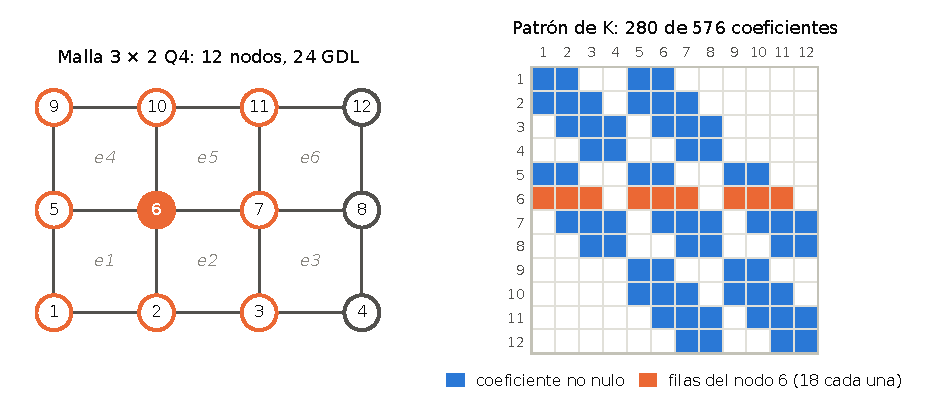
\includegraphics[width=\textwidth]{figuras/malla_patron.pdf}
  \caption{Por qué $\mK$ es dispersa. Izquierda: malla de $3\times2$ elementos Q4; el nodo~6 comparte elemento con los ocho nodos de borde naranja. Derecha: patrón de $\mK$ ($24\times24$, un bloque de $2\times2$ por cada par de nodos): el bloque $(i,j)$ es no nulo solo si los nodos $i$ y $j$ comparten un elemento. Las dos filas del nodo~6 tienen 18 coeficientes no nulos de 24; en una malla de miles de nodos seguirían teniendo 18. Se guardan \cifra{malla:nnz} coeficientes; algunos se anulan o casi porque los aportes de elementos vecinos se cancelan por simetría (\cifra{malla:ceros} dan cero exacto en punto flotante), y se guardan igual: el formato disperso sigue el \emph{patrón} que dicta la conectividad, no los valores.}
  \label{fig:patron}
\end{figure}

% ══════════════════════════════════════════════════════════════════════════
\section{¿Por qué no se invierte \texorpdfstring{$\bm{K}$}{K}?}\label{sec:inversa}

\subsection{\texorpdfstring{$\bm{u}=\bm{K}^{-1}\bm{F}$}{u = inv(K) F} es una notación, no un algoritmo}

La expresión $\bm{u}_f=\Kff^{-1}\bm{F}_f$ afirma que la solución existe y es única; no dice cómo calcularla. Con un escalar pasa lo mismo: para resolver $7x=21$ nadie calcula $7^{-1}=0{,}142857\ldots$ y después lo multiplica por 21 ---con seis decimales daría $2{,}999997$---; se divide y sale $3$. Con matrices, «dividir» es \emph{factorizar y sustituir}.

\subsection{La inversa de una matriz dispersa es llena}\label{sec:inversa-llena}

La inversa de la rigidez tiene significado físico: es la matriz de \textbf{flexibilidad}. Su columna $j$ resuelve $\mK\bm{c}_j=\bm{e}_j$, así que contiene los desplazamientos de todos los GDL cuando actúa una fuerza unitaria en el GDL $j$. En un cuerpo conectado, una fuerza aplicada en un punto desplaza, en general, todos los puntos. Por eso $\mK^{-1}$ es llena aunque $\mK$ sea casi toda ceros.

\begin{figure}[htbp]
\centering
\begin{tikzpicture}[x=1cm,y=1cm]
  \fill[pattern=north east lines,pattern color=tenue] (-0.3,-0.45) rectangle (0,0.45);
  \draw[line width=0.9pt,tinta] (0,-0.45) -- (0,0.45);
  \draw[resorte] (0,0) -- (1.55,0);   \node[font=\footnotesize] at (0.8,0.42) {$k$};
  \draw[resorte] (2.05,0) -- (3.55,0); \node[font=\footnotesize] at (2.8,0.42) {$k$};
  \draw[resorte] (4.05,0) -- (5.55,0); \node[font=\footnotesize] at (4.8,0.42) {$k$};
  \node[nodo] at (1.8,0) {1}; \node[nodo] at (3.8,0) {2}; \node[nodo] at (5.8,0) {3};
  \draw[-{Stealth[length=2.4mm]},line width=1pt,serie2] (6.08,0) -- (7.0,0) node[right,text=tinta] {$P$};
\end{tikzpicture}
\caption{Ejemplo 1: tres resortes iguales en serie, empotrados a la izquierda. Cada nodo tiene un GDL (el desplazamiento horizontal).}
\label{fig:cadena}
\end{figure}

\textbf{Ejemplo 1.} Para la cadena de la figura~\ref{fig:cadena},
\begin{equation}\label{eq:cadena}
\mK=k\begin{bmatrix}2&-1&0\\-1&2&-1\\0&-1&1\end{bmatrix},\qquad
\mK^{-1}=\frac1k\begin{bmatrix}1&1&1\\1&2&2\\1&2&3\end{bmatrix},\qquad
(\mK^{-1})_{ij}=\frac{\min(i,j)}{k}.
\end{equation}
La columna 3 de $\mK^{-1}$ dice que una fuerza unitaria en el nodo~3 desplaza los nodos 1, 2 y 3 en $1/k$, $2/k$ y $3/k$: cada resorte transmite la fuerza y se alarga $1/k$. $\mK$ tiene dos ceros ---los nodos 1 y 3 no están unidos por un resorte--- y $\mK^{-1}$ no tiene ninguno, porque una fuerza en el nodo~3 sí mueve al nodo~1. En cambio, los factores $\bm{L}$ y $\bm{U}$ de esta misma matriz (§\ref{sec:ejemplo1}) conservan los dos ceros. \emph{Factorizar preserva la dispersión; invertir la destruye.}

Medido con EduFEM en la membrana de Cook: con \cifra{q9:24:n} GDL libres, $\Kff$ tiene el \cifra{q9:24:densKr}\,\% de sus coeficientes no nulos y su inversa, el \cifra{q9:24:densInv}\,\% (\cifra{q9:24:cerosInv} ceros exactos).

\subsection{Costo en operaciones}

La tabla~\ref{tab:flops} cuenta las operaciones de punto flotante (\emph{flops}) de cada camino para una matriz densa de orden $n$; la deducción está en el apéndice~\ref{ap:flops}.

\begin{table}[htbp]
\centering
\caption{Operaciones para resolver $\mK\bm{u}=\bm{F}$ con una matriz densa de orden $n$.}
\label{tab:flops}
\begin{tabular}{lcc}
\toprule
Paso & Por factorización & Por inversa \\
\midrule
Factorizar $\mK=\bm{L}\bm{U}$ & $\tf23 n^3$ & $\tf23 n^3$ \\
Completar la inversa ($n$ sistemas triangulares) & --- & $\tf43 n^3$ \\
Sustituir ($\bm{L}\bm{y}=\bm{F}$, $\bm{U}\bm{u}=\bm{y}$) o multiplicar ($\mK^{-1}\bm{F}$) & $2n^2$ & $2n^2$ \\
\midrule
Total & $\approx\tf23 n^3$ & $\approx 2n^3$ \\
\bottomrule
\end{tabular}
\end{table}

Aun en formato denso, invertir cuesta tres veces más que factorizar. En formato disperso la brecha es mucho mayor. Con el mejor ordenamiento conocido para mallas planas, la disección anidada, la LU cuesta del orden de $n^{3/2}$ operaciones~\cite{george1973}; la inversa, con sus $n^2$ coeficientes, cuesta del orden de $n^3$. El mínimo grado que usa EduFEM no tiene la garantía de la disección anidada, y en estas mallas sus operaciones crecen algo más rápido: contadas sobre los factores que produce SuperLU (tabla~\ref{tab:llenado}), como $n^{\cifra{expo:flops}}$. Sigue estando muy lejos del $n^3$. Con \cifra{q9:64:n} GDL la factorización hace \cifra{q9:64:flops:MMD_AT_PLUS_A} operaciones, contra \cifra{q9:64:flopsDensa} de una LU densa ---unas \cifra{q9:64:xflopsDensa} veces más--- y \cifra{q9:64:flopsInv} de la inversa.

\subsection{Memoria}

Guardar $\mK^{-1}$ exige $8n^2$ bytes (8 por número en doble precisión). Con \cifra{q9:64:n} GDL son \cifra{q9:64:gbInv}~GB, más que toda la memoria del equipo en que se midieron estas cifras. Los factores $\bm{L}$ y $\bm{U}$ ordenados con mínimo grado tienen \cifra{q9:64:lu:MMD_AT_PLUS_A} coeficientes y ocupan unos \cifra{q9:64:mbLU}~MB (unos 12 bytes por coeficiente: 8 del valor y 4 del índice).

\subsection{Precisión}

Hay también un argumento de exactitud. La solución por LU y sustitución es \emph{regresivamente estable}: el $\hat{\bm{u}}$ calculado es la solución exacta de un sistema vecino $(\mK+\Delta\mK)\hat{\bm{u}}=\bm{F}$ con $\|\Delta\mK\|$ del orden del redondeo, $\varepsilon\|\mK\|$ ($\varepsilon\approx1{,}1\times10^{-16}$). Multiplicar por una inversa calculada no tiene esa garantía: su residuo $\bm{F}-\mK\hat{\bm{u}}$ puede ser hasta $\kappa(\mK)$ veces mayor~\cite{higham2002}. En la membrana de Cook la matriz está bien condicionada ---$\kappa_2(\Kff)\approx\cifra{q9:16:cond}$ con \cifra{q9:16:n} GDL--- y los tres caminos de la tabla~\ref{tab:denso} dan residuos relativos del orden de $10^{-12}$: aquí lo decisivo es el costo y la memoria. La precisión pasa a importar con matrices mal condicionadas: elementos muy distorsionados, coeficiente de Poisson cercano a 0,5 o materiales de rigideces muy dispares.

\begin{table}[htbp]
\centering
\caption{Tres maneras de resolver el mismo $\Kff\bm{u}_f=\bm{F}_f$ (membrana de Cook, Q9). \emph{SuperLU}: \cod{spsolve} con \ordMMD, como EduFEM. \emph{LU densa}: \cod{numpy.linalg.solve}, que también factoriza (LAPACK), pero sobre los $n^2$ coeficientes. \emph{Inversa}: \cod{numpy.linalg.inv(K) @ F}. Residuo: $\|\Kff\hat{\bm{u}}_f-\bm{F}_f\|_2/\|\bm{F}_f\|_2$. Tiempos: mejor de 15 corridas (SuperLU) y de 7, 4 y 2 (densos, de menor a mayor $n$).}
\label{tab:denso}
\small
\begin{tabular}{rrrrcccr}
\toprule
& \multicolumn{3}{c}{Tiempo (s)} & \multicolumn{3}{c}{Residuo relativo} & No nulos \\
\cmidrule(lr){2-4}\cmidrule(lr){5-7}
$n$ & SuperLU & LU densa & Inversa & SuperLU & LU densa & Inversa & de $\Kff^{-1}$ \\
\midrule
\filas{datos/tabla_denso.tex}
\bottomrule
\end{tabular}
\end{table}

Con \cifra{q9:24:n} GDL, la inversa tarda \cifra{q9:24:tinv}~s y SuperLU \cifra{q9:24:t:MMD_AT_PLUS_A}~s: \cifra{q9:24:xinv} veces más. Incluso frente a la LU densa de NumPy, la inversa es \cifra{q9:24:xinvsolve} veces más lenta, cerca de la razón teórica de 3 de la tabla~\ref{tab:flops}.

\begin{ojo}[title={¿Dónde sí invierte algo EduFEM?}]
Solo en matrices pequeñas de tamaño fijo: el Jacobiano $2\times2$ de cada punto de Gauss, por la fórmula cerrada de cofactores (\cod{fem/batch.py}, líneas 189--195), y la matriz de extrapolación de tensiones de los puntos de Gauss a los nodos, de $4\times4$ en Q4 y $9\times9$ en Q9, que es una constante del tipo de elemento (\cod{fem/stress.py}, línea 131). La matriz de rigidez no se invierte nunca.
\end{ojo}

% ══════════════════════════════════════════════════════════════════════════
\section{Factorización LU}\label{sec:lu}

\subsection{La eliminación de Gauss, escrita como un producto}

Resolver $\bm{A}\bm{x}=\bm{b}$ por eliminación de Gauss~\cite{golub2013,trefethen1997} es anular, columna por columna, los coeficientes que quedan debajo de la diagonal. En el paso $k$ el pivote es $a_{kk}^{(k)}$ y cada fila $i>k$ se modifica así:
\begin{equation}\label{eq:multiplicador}
\ell_{ik}=\frac{a_{ik}^{(k)}}{a_{kk}^{(k)}},\qquad
a_{ij}^{(k+1)}=a_{ij}^{(k)}-\ell_{ik}\,a_{kj}^{(k)}\qquad(j=k,\dots,n),
\end{equation}
lo que deja $a_{ik}^{(k+1)}=0$. Tras $n-1$ pasos queda una matriz triangular superior, $\bm{U}=\bm{A}^{(n)}$. Si los multiplicadores $\ell_{ik}$ se guardan en una matriz triangular inferior con unos en la diagonal, $\bm{L}$, se cumple
\begin{equation}\label{eq:lu}
\boxed{\;\bm{A}=\bm{L}\,\bm{U}\;}
\end{equation}
La razón: el paso $k$ equivale a multiplicar por la izquierda por $\bm{M}_k=\bm{I}-\bm{\ell}_k\bm{e}_k\T$, donde el vector $\bm{\ell}_k$ contiene los multiplicadores de la columna $k$. Entonces $\bm{U}=\bm{M}_{n-1}\cdots\bm{M}_1\bm{A}$, es decir, $\bm{A}=\bm{M}_1^{-1}\cdots\bm{M}_{n-1}^{-1}\bm{U}$. Cada inversa $\bm{M}_k^{-1}=\bm{I}+\bm{\ell}_k\bm{e}_k\T$ se obtiene cambiando un signo, y su producto es la matriz $\bm{L}$ con cada multiplicador en su lugar. \emph{$\bm{L}$ sale gratis de la eliminación}: no hay que calcular nada más.

\begin{lstlisting}[style=algo,title={\textbf{Algoritmo 1.} LU sin pivoteo (Doolittle), sobre el propio arreglo $\bm{A}$.}]
para k = 1, ..., n-1
    para i = k+1, ..., n              (solo filas con $a_{ik}$ ≠ 0)
        ℓ[i,k] ← a[i,k] / a[k,k]
        para j = k+1, ..., n          (solo columnas con $a_{kj}$ ≠ 0)
            a[i,j] ← a[i,j] − ℓ[i,k] · a[k,j]
\end{lstlisting}

Los dos comentarios entre paréntesis resumen toda la LU dispersa: si $a_{ik}=0$ no hay multiplicador que calcular, y si $a_{kj}=0$ no hay nada que actualizar.

\subsection{Ejemplo 1, paso a paso: la cadena de resortes}\label{sec:ejemplo1}

Se factoriza $\bm{A}=\mK/k$ de la ecuación~\eqref{eq:cadena} y al final se divide por $k$. El sistema es $\mK\bm{u}=(0,0,P)\T$.

\begin{paso}[title={Paso 1: pivote $a_{11}=2$}]
Fila 2: $\ell_{21}=\dfrac{-1}{2}=-\tf12$;\quad $a_{22}\leftarrow 2-\bigl(-\tf12\bigr)(-1)=\tf32$;\quad $a_{23}\leftarrow -1-\bigl(-\tf12\bigr)(0)=-1$.\\
Fila 3: $a_{31}=0$, así que $\ell_{31}=0$ y la fila no se toca. Aquí la dispersión ya ahorra trabajo.
\[
\bm{A}^{(2)}=\begin{bmatrix}2&-1&0\\0&\tf32&-1\\0&-1&1\end{bmatrix}
\]
\end{paso}

\begin{paso}[title={Paso 2: pivote $a_{22}=\tf32$}]
Fila 3: $\ell_{32}=\dfrac{-1}{3/2}=-\tf23$;\quad $a_{33}\leftarrow 1-\bigl(-\tf23\bigr)(-1)=\tf13$.
\[
\bm{L}=\begin{bmatrix}1&0&0\\-\tf12&1&0\\0&-\tf23&1\end{bmatrix},\qquad
\bm{U}=\begin{bmatrix}2&-1&0\\0&\tf32&-1\\0&0&\tf13\end{bmatrix}.
\]
Comprobación de la fila 3 de $\bm{L}\bm{U}$: $0\cdot(2,-1,0)-\tf23\bigl(0,\tf32,-1\bigr)+1\cdot\bigl(0,0,\tf13\bigr)=(0,-1,1)$, que es la fila 3 de $\bm{A}$.
\end{paso}

\begin{paso}[title={Paso 3: sustitución hacia adelante, $\bm{L}\bm{y}=\bm{b}$, con $\bm{b}=(0,0,P/k)$}]
$y_1=0$;\quad $y_2=0-\bigl(-\tf12\bigr)y_1=0$;\quad $y_3=\dfrac{P}{k}-\bigl(-\tf23\bigr)y_2=\dfrac{P}{k}$.
\end{paso}

\begin{paso}[title={Paso 4: sustitución hacia atrás, $\bm{U}\bm{u}=\bm{y}$}]
$u_3=\dfrac{P/k}{1/3}=\dfrac{3P}{k}$;\quad
$u_2=\dfrac{0-(-1)\,u_3}{3/2}=\dfrac{2P}{k}$;\quad
$u_1=\dfrac{0-(-1)\,u_2}{2}=\dfrac{P}{k}$.
\end{paso}

\begin{resultado}[title={Lo que muestra el ejemplo}]
\begin{itemize}[leftmargin=1.2em]
  \item Comprobación física: cada resorte transmite $P$ y se alarga $P/k$; en efecto $u_1-0=u_2-u_1=u_3-u_2=P/k$.
  \item Los ceros $a_{13}=a_{31}=0$ de $\mK$ siguen siendo ceros en $\bm{L}$ y $\bm{U}$: esta factorización no creó ningún coeficiente nuevo. Con $n$ resortes en serie, $\mK$ tiene $3n-2$ no nulos, $\bm{L}+\bm{U}$ los mismos $3n-2$ y $\mK^{-1}$, $n^2$.
  \item Los pivotes $2$, $\tf32$ y $\tf13$ son positivos y su producto es $\det\bm{A}=1$.
\end{itemize}
\end{resultado}

\subsection{Sustitución hacia adelante y hacia atrás}

En general,
\begin{align}
y_i&=b_i-\sum_{j<i}\ell_{ij}\,y_j, & i&=1,2,\dots,n, \label{eq:adelante}\\
x_i&=\frac{1}{u_{ii}}\Bigl(y_i-\sum_{j>i}u_{ij}\,x_j\Bigr), & i&=n,n-1,\dots,1. \label{eq:atras}
\end{align}
Cada sustitución recorre una sola vez los coeficientes de su factor: $\approx n^2$ operaciones en denso y $\approx2\nnz$ en disperso. Es la parte barata.

\subsection{¿Por qué factorizar?}

\begin{itemize}
  \item \textbf{Separa lo caro de lo barato.} Factorizar se hace una vez; sustituir, una vez por cada vector de cargas. Con varios estados de carga, $\bm{L}$ y $\bm{U}$ se reutilizan (§\ref{sec:spsolve-splu}).
  \item \textbf{Diagnostica.} $\det\mK=\prod_k u_{kk}$ (con pivoteo, salvo el signo de la permutación). Un pivote nulo delata una $\Kff$ singular, es decir, un \emph{mecanismo}: el modelo no está bien restringido. SuperLU lo detecta, SciPy devuelve \cod{NaN} y EduFEM lo informa (\cod{fem/solver.py}, líneas 134--139).
  \item \textbf{Conserva la dispersión} si las incógnitas se ordenan bien (§\ref{sec:llenado}), cosa que la inversa no puede hacer.
\end{itemize}

\subsection{Pivoteo, y por qué una matriz SPD no lo necesita}\label{sec:pivoteo}

La fórmula~\eqref{eq:multiplicador} divide por el pivote. Con $\bm{A}=\bigl[\begin{smallmatrix}0&1\\1&1\end{smallmatrix}\bigr]$ el primer pivote es cero y el algoritmo se detiene, aunque $\bm{A}$ es invertible; con $\bigl[\begin{smallmatrix}\epsilon&1\\1&1\end{smallmatrix}\bigr]$ y $\epsilon$ diminuto, el multiplicador $1/\epsilon$ es enorme y amplifica el redondeo. La cura general es el \textbf{pivoteo parcial}: en el paso $k$ se intercambia la fila $k$ con la de mayor $|a_{ik}|$, y se obtiene $\bm{P}\bm{A}=\bm{L}\bm{U}$ con $|\ell_{ik}|\le1$.

Una matriz SPD no lo necesita, por dos razones:
\begin{enumerate}
  \item \textbf{Los pivotes son positivos.} $u_{kk}=\det\bm{A}_k/\det\bm{A}_{k-1}$, donde $\bm{A}_k$ es la submatriz principal de orden $k$; toda submatriz principal de una SPD es SPD y tiene determinante positivo. En el ejemplo 1, $\det\bm{A}_1=2$, $\det\bm{A}_2=3$ y $\det\bm{A}_3=1$, y los pivotes son $2/1$, $3/2$ y $1/3$.
  \item \textbf{Los números no crecen.} Al eliminar, la diagonal de la parte que falta factorizar solo puede disminuir, $a_{ii}^{(k+1)}=a_{ii}^{(k)}-\bigl(a_{ik}^{(k)}\bigr)^2/a_{kk}^{(k)}\le a_{ii}^{(k)}$, y en una SPD cada coeficiente está acotado por la diagonal, $|a_{ij}|\le\sqrt{a_{ii}\,a_{jj}}$. Ningún coeficiente intermedio ---ni de $\bm{U}$--- supera al mayor coeficiente diagonal de la matriz original, y la eliminación sin pivoteo es estable~\cite{higham2002}.
\end{enumerate}
Esto permite elegir el orden de eliminación \emph{solo} por la dispersión, sin preocuparse por la estabilidad (§\ref{sec:llenado} y~\ref{sec:md}). SuperLU, que es un código general, pivotea igual, pero con un umbral que favorece la diagonal (§\ref{sec:umbral}).

\subsection{Cholesky y \texorpdfstring{$\bm{L}\bm{D}\bm{L}^{\top}$}{LDLT}}\label{sec:cholesky}

Si $\bm{A}$ es simétrica, $\bm{U}$ no aporta información nueva: $\bm{U}=\bm{D}\bm{L}\T$ con $\bm{D}=\operatorname{diag}(u_{11},\dots,u_{nn})$, y entonces $\bm{A}=\bm{L}\bm{D}\bm{L}\T$. En el ejemplo 1, $\bm{D}=\operatorname{diag}\bigl(2,\tf32,\tf13\bigr)$, y $\bm{D}\bm{L}\T$ reproduce $\bm{U}$ fila por fila; la fila 2, por ejemplo, es $\tf32\cdot\bigl(0,1,-\tf23\bigr)=\bigl(0,\tf32,-1\bigr)$. Si además $\bm{A}$ es definida positiva, $\bm{D}$ tiene raíz y $\bm{A}=\bm{G}\bm{G}\T$ con $\bm{G}=\bm{L}\bm{D}^{1/2}$: es la \textbf{factorización de Cholesky}. Para el ejemplo 1,
\[
\bm{G}=\begin{bmatrix}\sqrt2&0&0\\-1/\sqrt2&\sqrt{3/2}&0\\0&-\sqrt{2/3}&1/\sqrt3\end{bmatrix}.
\]
Cholesky hace la mitad de las operaciones ($n^3/3$ en denso) y guarda un solo triángulo. EduFEM usa, sin embargo, la LU general de SuperLU por una razón práctica: SciPy no incluye una factorización de Cholesky dispersa ---la de referencia, CHOLMOD, llega a Python con \cod{scikit-sparse}, una dependencia binaria más que habría que empaquetar en el instalador---; la tesis la deja como recomendación. La diferencia es un factor constante, cercano a 2 en operaciones y en memoria, y no un cambio de orden de magnitud: con el ordenamiento simétrico de la sección~\ref{sec:md} y pivotes diagonales, $\bm{U}$ tiene el mismo patrón que $\bm{L}\T$. Medido con \cifra{q9:64:n} GDL: $\nnz(\bm{L})=\cifra{q9:64:nnzL}$ y $\nnz(\bm{U})=\cifra{q9:64:nnzU}$.

% ══════════════════════════════════════════════════════════════════════════
\section{Matrices dispersas: COO, CSR y CSC}\label{sec:disperso}

\subsection{Guardar solo lo que no es cero}

Una matriz densa de orden $n$ ocupa $8n^2$ bytes, ceros incluidos. Con \cifra{q9:64:n} GDL libres, $\Kff$ densa ocuparía \cifra{q9:64:gbInv}~GB; en formato disperso ocupa \cifra{q9:64:mbKr}~MB. Los formatos dispersos guardan solo los coeficientes no nulos, cada uno acompañado de la información necesaria para saber dónde va~\cite{davis2006}. SciPy ofrece varios~\cite{virtanen2020}; EduFEM usa tres.

\subsection{COO: la lista de tripletes}\label{sec:coo}

El formato de coordenadas (\emph{coordinate list}, COO) guarda tres arreglos de la misma longitud: \cod{row}, \cod{col} y \cod{data}. El coeficiente número $m$ es el triplete $(\text{\cod{row}}[m],\text{\cod{col}}[m],\text{\cod{data}}[m])$. Dos propiedades lo hacen ideal para ensamblar:
\begin{itemize}
  \item el orden de los tripletes no importa;
  \item \textbf{puede haber tripletes repetidos en la misma posición $(i,j)$, y al convertir la matriz a otro formato (o al operar con ella) se suman}.
\end{itemize}
La segunda propiedad \emph{es} el ensamblaje~\eqref{eq:ensamblaje}: basta con listar todos los aportes elementales, cada uno en su posición global, y la conversión hace el «$+{=}$».

\begin{figure}[htbp]
\centering
\begin{tikzpicture}[x=1cm,y=1cm]
  \draw[line width=2.4pt,serie1!75] (0,0) -- (4,0);
  \draw[line width=2.4pt,serie3!85!black] (4,0) -- (8,0);
  \node[nodo] at (0,0) {0}; \node[nodo] at (4,0) {1}; \node[nodo] at (8,0) {2};
  \node[font=\footnotesize,text=serie1!75!black] at (2,0.42) {elemento 1: GDL $(0,1)$};
  \node[font=\footnotesize,text=serie3!60!black] at (6,0.42) {elemento 2: GDL $(1,2)$};
\end{tikzpicture}
\caption{Ejemplo 4: barra de dos elementos con un GDL por nodo, numerados desde 0 como en el código. Cada elemento tiene $\bm{k}_e=k\bigl[\begin{smallmatrix}1&-1\\-1&1\end{smallmatrix}\bigr]$ con $k=EA/L$.}
\label{fig:barra}
\end{figure}

\textbf{Ejemplo 4.} Para la barra de la figura~\ref{fig:barra}, cada elemento aporta sus cuatro coeficientes:

\begin{center}
\small
\begin{tabular}{ccccl}
\toprule
$m$ & \cod{row} & \cod{col} & \cod{data} & origen \\
\midrule
0 & 0 & 0 & $k$  & elemento 1, $(\bm{k}_e)_{11}$ \\
1 & 0 & 1 & $-k$ & elemento 1, $(\bm{k}_e)_{12}$ \\
2 & 1 & 0 & $-k$ & elemento 1, $(\bm{k}_e)_{21}$ \\
\rowcolor{serie2!10}
3 & 1 & 1 & $k$  & elemento 1, $(\bm{k}_e)_{22}$ \\
\rowcolor{serie2!10}
4 & 1 & 1 & $k$  & elemento 2, $(\bm{k}_e)_{11}$ \\
5 & 1 & 2 & $-k$ & elemento 2, $(\bm{k}_e)_{12}$ \\
6 & 2 & 1 & $-k$ & elemento 2, $(\bm{k}_e)_{21}$ \\
7 & 2 & 2 & $k$  & elemento 2, $(\bm{k}_e)_{22}$ \\
\bottomrule
\end{tabular}
\end{center}

Los tripletes 3 y 4 caen en la misma posición $(1,1)$ y se suman: $k+k=2k$. El nodo 1 pertenece a los dos elementos y recibe la rigidez de ambos:
\[
\mK=k\begin{bmatrix}1&-1&0\\-1&2&-1\\0&-1&1\end{bmatrix}.
\]

\subsection{CSR: filas comprimidas}

El formato de filas comprimidas (\emph{compressed sparse row}, CSR) guarda los valores fila por fila en \cod{data}, la columna de cada valor en \cod{indices}, y un arreglo \cod{indptr} de longitud $n+1$ que marca dónde empieza cada fila: la fila $i$ ocupa las posiciones $\text{\cod{indptr}}[i],\dots,\text{\cod{indptr}}[i+1]-1$. Para la barra:
\[
\begin{aligned}
\text{\cod{indptr}}&=[\,0,\;2,\;5,\;7\,]\\
\text{\cod{indices}}&=[\,0,1,\;\;0,1,2,\;\;1,2\,]\\
\text{\cod{data}}&=[\,k,-k,\;\;-k,2k,-k,\;\;-k,k\,]
\end{aligned}
\]
Para leer la fila 1 se toman las posiciones 2 a 4: columnas $0,1,2$ con valores $-k,2k,-k$. Recorrer una fila cuesta tanto como sus no nulos, y la memoria es $\approx12\nnz$ bytes (8 del valor y 4 del índice) más $4(n+1)$ de \cod{indptr}.

\subsection{CSC: columnas comprimidas}

El formato de columnas comprimidas (\emph{compressed sparse column}, CSC) es lo mismo por columnas: \cod{indptr} marca dónde empieza cada columna e \cod{indices} guarda filas. Como $\mK$ es simétrica, sus arreglos CSC son idénticos a los CSR ---para la barra, el guion lo verifica---, pero el formato indica al programa cómo recorrerlos. SuperLU trabaja columna por columna (§\ref{sec:izquierda}), así que su formato nativo es CSC.

\subsection{Qué formato para qué}

\begin{center}
\small
\begin{tabularx}{\textwidth}{l>{\raggedright\arraybackslash}X>{\raggedright\arraybackslash}X}
\toprule
Formato & Bueno para & Dónde lo usa EduFEM \\
\midrule
COO & construir: agregar tripletes en cualquier orden, con repetidos & \cod{assemble_sparse} (\cod{fem/batch.py}) \\
CSR & recorrer y extraer filas; producto $\mK\bm{u}$ & $\mK$ global; submatriz $\Kff$; reacciones $\mK[r,:]\,\bm{u}$ \\
CSC & recorrer y extraer columnas; algoritmos por columnas & $\Kff$ justo antes de SuperLU (\cod{K_red.tocsc()}) \\
\bottomrule
\end{tabularx}
\end{center}

\subsection{El ensamblaje de EduFEM, línea por línea}

\begin{lstlisting}[style=py,firstnumber=234,caption={\cod{fem/batch.py}: el ensamblaje completo de $\mK$.}]
def assemble_sparse(dofs, ke, n_dof):
    """Scatter local -> global como tripletes COO y conversion a CSR.

    `coo_matrix` suma las entradas duplicadas en la misma (i, j): es
    exactamente la suma de contribuciones elementales del MEF. K nunca se
    materializa densa (memoria O(nnz)).
    """
    dofs = np.asarray(dofs, dtype=np.intp)
    n_dof_e = dofs.shape[1] if dofs.ndim == 2 else 0
    rows = np.repeat(dofs, n_dof_e, axis=1).ravel()   # [i0, i0, ..., i1, i1, ...]
    cols = np.tile(dofs, (1, n_dof_e)).ravel()        # [j0, j1, ..., j0, j1, ...]
    data = np.asarray(ke, dtype=float).ravel()
    return coo_matrix((data, (rows, cols)), shape=(n_dof, n_dof)).tocsr()
\end{lstlisting}

\cod{dofs} es un arreglo de $e\times 2n_e$ con los GDL globales de cada elemento ($2n_e=8$ en Q4 y 18 en Q9) y \cod{ke} es el lote de rigideces, de $e\times2n_e\times2n_e$. Con la barra, \cod{dofs = [[0, 1], [1, 2]]} y:
\begin{itemize}
  \item \cod{np.repeat(dofs, 2, axis=1).ravel()} repite cada GDL tantas veces como columnas tiene $\bm{k}_e$: \cod{[0,0,1,1, 1,1,2,2]}, la columna \cod{row} de la tabla anterior;
  \item \cod{np.tile(dofs, (1, 2)).ravel()} repite la lista entera de GDL del elemento una vez por fila de $\bm{k}_e$: \cod{[0,1,0,1, 1,2,1,2]}, la columna \cod{col};
  \item \cod{ke.ravel()} aplana las matrices elementales fila por fila: \cod{[k,-k,-k,k, k,-k,-k,k]}, la columna \cod{data}.
\end{itemize}
El triplete $m=e\,(2n_e)^2+a\,(2n_e)+b$ lleva $(\bm{k}_e)_{ab}$ a la posición global $(\text{\cod{dofs}}[e,a],\text{\cod{dofs}}[e,b])$: es el operador $\bm{A}_e\T\bm{k}_e\bm{A}_e$ de la ecuación~\eqref{eq:ensamblaje} sin construir ninguna $\bm{A}_e$. Finalmente, \cod{coo_matrix((data, (rows, cols)), ...)} arma la matriz COO y \cod{.tocsr()} la convierte a CSR sumando los repetidos. El guion verifica que esta misma función, aplicada a la barra, devuelve exactamente los arreglos \cod{indptr}, \cod{indices} y \cod{data} de arriba.

Con la membrana de Cook de $8\times8$ elementos Q9 hay \cifra{q9:8:elementos} elementos $\times\,18^2$ = \cifra{q9:8:tripletes} tripletes; al sumar los \cifra{q9:8:duplicados} repetidos quedan \cifra{q9:8:nnzK} coeficientes en $\mK$. Con $64\times64$ elementos, \cifra{q9:64:tripletes} tripletes se reducen a \cifra{q9:64:nnzK} coeficientes.

\begin{clave}[title={Quién hace qué en el ensamblaje}]
\textbf{NumPy} calcula el lote de $\bm{k}_e$ (\cod{einsum}, \cod{matmul} en \cod{stiffness_batch}) y arma \cod{rows}, \cod{cols} y \cod{data} con \cod{repeat}, \cod{tile} y \cod{ravel}: bucles en C, sin un bucle de Python por elemento. \textbf{SciPy} (\cod{scipy.sparse}) construye la matriz COO y la convierte a CSR, también en código compilado; la suma de repetidos ocurre ahí. La matriz nunca existe en forma densa.
\end{clave}

% ══════════════════════════════════════════════════════════════════════════
\section{El llenado: por qué importa el orden de las incógnitas}\label{sec:llenado}

\subsection{Qué es el llenado}

Se llama \textbf{llenado} (\emph{fill-in}) a los coeficientes que son cero en la matriz y dejan de serlo en $\bm{L}$ o en $\bm{U}$. Aparecen por la actualización~\eqref{eq:multiplicador}: si $a_{ij}=0$ pero $\ell_{ik}\neq0$ y $a_{kj}\neq0$, entonces $a_{ij}-\ell_{ik}a_{kj}\neq0$. Cada coeficiente de llenado ocupa memoria y, peor, participa en todas las actualizaciones posteriores. En la cadena de resortes no hubo llenado; el ejemplo siguiente muestra que la misma física puede generar mucho o nada, según el orden.

\subsection{Ejemplo 2: una estrella}\label{sec:estrella}

Un nodo central (1) está unido por resortes de rigidez 1 a tres nodos periféricos (2, 3 y 4), y cada nodo está además anclado a tierra: el central con un resorte de rigidez 1 y los periféricos con resortes de rigidez 2. Con fuerzas $\bm{F}=(1,2,2,2)$:
\[
\mK=\begin{bmatrix}4&-1&-1&-1\\-1&3&0&0\\-1&0&3&0\\-1&0&0&3\end{bmatrix},\qquad
\bm{F}=\begin{bmatrix}1\\2\\2\\2\end{bmatrix},\qquad
\bm{u}=\begin{bmatrix}1\\1\\1\\1\end{bmatrix}.
\]
(Todos los nodos se desplazan 1: los resortes entre nodos no se estiran y cada anclaje toma su propia fuerza.) $\mK$ tiene 10 coeficientes no nulos de 16.

\begin{paso}[title={Orden A: el nodo central primero}]
\emph{Paso 1}, pivote $4$: $\ell_{21}=\ell_{31}=\ell_{41}=-\tf14$. Para $i,j\in\{2,3,4\}$, $a_{ij}\leftarrow a_{ij}-\bigl(-\tf14\bigr)(-1)=a_{ij}-\tf14$: la diagonal pasa de $3$ a $\tf{11}4$ y \textbf{los seis ceros se vuelven $-\tf14$}:
\[
\bm{A}^{(2)}=\begin{bmatrix}4&-1&-1&-1\\0&\tf{11}4&\rel{-\tf14}&\rel{-\tf14}\\0&\rel{-\tf14}&\tf{11}4&\rel{-\tf14}\\0&\rel{-\tf14}&\rel{-\tf14}&\tf{11}4\end{bmatrix}.
\]
\emph{Paso 2}, pivote $\tf{11}4$: $\ell_{32}=\ell_{42}=\dfrac{-1/4}{11/4}=-\tf1{11}$; $a_{33}\leftarrow\tf{11}4-\tf1{44}=\tf{30}{11}$; $a_{34}\leftarrow-\tf14-\tf1{44}=-\tf3{11}$ (y lo mismo en la fila 4).\\
\emph{Paso 3}, pivote $\tf{30}{11}$: $\ell_{43}=\dfrac{-3/11}{30/11}=-\tf1{10}$; $a_{44}\leftarrow\tf{30}{11}-\tf3{110}=\tf{27}{10}$.
\[
\bm{L}=\begin{bmatrix}1&&&\\-\tf14&1&&\\-\tf14&\rel{-\tf1{11}}&1&\\-\tf14&\rel{-\tf1{11}}&\rel{-\tf1{10}}&1\end{bmatrix},\qquad
\bm{U}=\begin{bmatrix}4&-1&-1&-1\\&\tf{11}4&\rel{-\tf14}&\rel{-\tf14}\\&&\tf{30}{11}&\rel{-\tf3{11}}\\&&&\tf{27}{10}\end{bmatrix}.
\]
$\bm{L}+\bm{U}$ tiene los 16 coeficientes llenos: \textbf{6 de llenado} (en naranja).
\end{paso}

\begin{paso}[title={Orden B: el nodo central al final}]
Se renumeran los nodos como $(2,3,4,1)$, es decir, se factoriza $\bm{P}\mK\bm{P}\T$:
\[
\bm{P}\mK\bm{P}\T=\begin{bmatrix}3&0&0&-1\\0&3&0&-1\\0&0&3&-1\\-1&-1&-1&4\end{bmatrix}.
\]
\emph{Paso 1}, pivote $3$: solo la fila 4 tiene un no nulo en la columna 1, $\ell_{41}=-\tf13$, y $a_{44}\leftarrow4-\bigl(-\tf13\bigr)(-1)=\tf{11}3$. La fila 1 tiene ceros en las columnas 2 y 3, así que no se crea nada.\\
\emph{Pasos 2 y 3}, iguales: $\ell_{42}=\ell_{43}=-\tf13$, y $a_{44}$ baja a $\tf{10}3$ y después a $3$.
\[
\bm{L}=\begin{bmatrix}1&&&\\0&1&&\\0&0&1&\\-\tf13&-\tf13&-\tf13&1\end{bmatrix},\qquad
\bm{U}=\begin{bmatrix}3&0&0&-1\\&3&0&-1\\&&3&-1\\&&&3\end{bmatrix}.
\]
$\bm{L}+\bm{U}$ tiene 10 coeficientes, los mismos de $\mK$: \textbf{ningún llenado}.
\end{paso}

Los dos órdenes resuelven el mismo problema. En el orden B, la sustitución hacia adelante con $\bm{P}\bm{F}=(2,2,2,1)$ da $\bm{y}=(2,2,2,3)$, y hacia atrás, $u=1$ en los cuatro nodos. Los determinantes también coinciden: $4\cdot\tf{11}4\cdot\tf{30}{11}\cdot\tf{27}{10}=81=3^4$.

\subsection{Renumerar es permutar}

Cambiar el orden de las incógnitas equivale a multiplicar por una matriz de permutación $\bm{P}$ (la identidad con las filas reordenadas), que cumple $\bm{P}\T\bm{P}=\bm{I}$:
\begin{equation}\label{eq:permutacion}
\mK\bm{u}=\bm{F}\iff\bigl(\bm{P}\mK\bm{P}\T\bigr)\bigl(\bm{P}\bm{u}\bigr)=\bm{P}\bm{F}.
\end{equation}
La física no cambia: solo cambia en qué orden se eliminan las ecuaciones. En EduFEM la numeración de los nodos es la que haya dejado el usuario ---el orden de los clics en el lienzo, el del archivo DXF importado, y en Q9 los nodos intermedios que \cod{expand_q4_to_q9} agrega al final---, así que el solucionador no puede confiar en ella. Reordena por su cuenta.

\subsection{El grafo de la matriz}\label{sec:grafo}

La herramienta para razonar sobre el llenado es el grafo de la matriz~\cite{george1981,davis2006}: un vértice por incógnita y una arista $\{i,j\}$ por cada coeficiente $K_{ij}\neq0$ con $i\neq j$. En el MEF ese grafo es, esencialmente, la \emph{conectividad de la malla}: dos nodos son vecinos si comparten un elemento.

\begin{clave}[title={Regla de eliminación en el grafo~\cite{parter1961,rose1972}}]
Eliminar la incógnita $v$ equivale, en el grafo, a \textbf{unir entre sí a todos los vecinos de $v$} (forman un bloque totalmente conectado) y quitar $v$. Las aristas nuevas son exactamente el llenado. Si $v$ tiene $d$ vecinos, se crean como mucho $d(d-1)/2$ aristas, y la eliminación cuesta del orden de $d^2$ operaciones.
\end{clave}

\begin{figure}[htbp]
\centering
\begin{minipage}[t]{0.3\textwidth}\centering
\begin{tikzpicture}[x=1cm,y=1cm]
  \coordinate (h) at (0,0); \coordinate (a) at (90:1.05); \coordinate (b) at (210:1.05); \coordinate (c) at (330:1.05);
  \draw[arista] (h) -- (a); \draw[arista] (h) -- (b); \draw[arista] (h) -- (c);
  \node[nodo] at (h) {1}; \node[nodo] at (a) {2}; \node[nodo] at (b) {3}; \node[nodo] at (c) {4};
\end{tikzpicture}
\par\smallskip{\footnotesize (a) Grafo de $\mK$: el nodo 1 tiene grado 3; los demás, grado 1.}
\end{minipage}\hfill
\begin{minipage}[t]{0.3\textwidth}\centering
\begin{tikzpicture}[x=1cm,y=1cm]
  \coordinate (h) at (0,0); \coordinate (a) at (90:1.05); \coordinate (b) at (210:1.05); \coordinate (c) at (330:1.05);
  \draw[relleno] (a) -- (b); \draw[relleno] (b) -- (c); \draw[relleno] (c) -- (a);
  \node[nodoelim] at (h) {1}; \node[nodo] at (a) {2}; \node[nodo] at (b) {3}; \node[nodo] at (c) {4};
\end{tikzpicture}
\par\smallskip{\footnotesize (b) Eliminar 1 une a sus tres vecinos: 3 aristas nuevas, los 6 coeficientes naranjas del orden A.}
\end{minipage}\hfill
\begin{minipage}[t]{0.3\textwidth}\centering
\begin{tikzpicture}[x=1cm,y=1cm]
  \coordinate (h) at (0,0); \coordinate (a) at (90:1.05); \coordinate (b) at (210:1.05); \coordinate (c) at (330:1.05);
  \draw[arista] (h) -- (b); \draw[arista] (h) -- (c);
  \node[nodo] at (h) {1}; \node[nodoelim] at (a) {2}; \node[nodo] at (b) {3}; \node[nodo] at (c) {4};
\end{tikzpicture}
\par\smallskip{\footnotesize (c) Eliminar una hoja (2) no crea nada: tiene un solo vecino. Es el orden B.}
\end{minipage}
\caption{El ejemplo 2 en el lenguaje de grafos. Líneas grises: coeficientes de $\mK$; naranja discontinuo: llenado; círculo punteado: incógnita ya eliminada.}
\label{fig:estrella}
\end{figure}

\subsection{¿Cuál es el mejor orden?}

Encontrar el orden de menor llenado es un problema NP-completo~\cite{yannakakis1981}: con miles de incógnitas no se puede buscar el óptimo, así que se usan heurísticas. Hay tres familias clásicas~\cite{davis2016}:
\begin{itemize}
  \item \textbf{Reducción del ancho de banda} (Cuthill--McKee y su versión inversa, RCM): numera de modo que los no nulos queden cerca de la diagonal; el llenado queda confinado dentro de la banda. EduFEM lo probó y lo retiró el 2026-09-06, porque el mínimo grado ya daba la ganancia grande (\cod{docs/convenciones/roadmap-fem.md}, ítem 3).
  \item \textbf{Mínimo grado}: una regla local y voraz que ataca el llenado directamente. Es la que usa EduFEM (§\ref{sec:md}).
  \item \textbf{Disección anidada}: parte la malla recursivamente con separadores y los numera al final; en mallas planas alcanza el orden de magnitud óptimo, $O(n\log n)$ de llenado y $O(n^{3/2})$ operaciones~\cite{george1973}.
\end{itemize}

% ══════════════════════════════════════════════════════════════════════════
\section{Ordenamiento de mínimo grado sobre \texorpdfstring{$\bm{K}^{\top}+\bm{K}$}{KT+K}}\label{sec:md}

\subsection{La regla}

El \textbf{grado} de un vértice es su número de vecinos en el grafo \emph{actual} de eliminación; en la matriz, es el número de no nulos fuera de la diagonal en su fila de la parte que falta factorizar. Como eliminar un vértice de grado $d$ crea hasta $d(d-1)/2$ aristas y cuesta $\approx d^2$ operaciones, la regla del mínimo grado~\cite{markowitz1957,tinney1967} es simple: \emph{eliminar siempre un vértice de grado mínimo}, actualizar el grafo y repetir.

\begin{lstlisting}[style=algo,title={\textbf{Algoritmo 2.} Mínimo grado.}]
G ← grafo de K
para k = 1, ..., n
    v ← un vértice de G con grado mínimo     (empates: el de menor número)
    π(k) ← v                                  (v será la incógnita k-ésima)
    unir entre sí a todos los vecinos de v    (aristas de llenado)
    quitar v de G
\end{lstlisting}

El resultado es una permutación $\pi$, es decir, una matriz $\bm{P}$ para la ecuación~\eqref{eq:permutacion}. El algoritmo trabaja \emph{solo con el patrón} de la matriz, nunca con sus valores, y termina antes de que empiece la factorización numérica.

\subsection{Ejemplo 3, paso a paso: una malla de \texorpdfstring{$2\times2$}{2x2} elementos Q4}\label{sec:ejemplo3}

La malla tiene 9 nodos numerados por filas (1--2--3 abajo, 7--8--9 arriba). Cada elemento une a sus cuatro nodos entre sí, así que el grafo tiene 20 aristas: cada nodo de esquina tiene grado 3, cada nodo de lado, grado 5, y el central, grado 8. Para que el ejemplo se pueda seguir a mano se trabaja con los nodos; la sección~\ref{sec:nodos-gdl} explica por qué con dos GDL por nodo el resultado es el mismo. La figura~\ref{fig:md-pasos} y la tabla~\ref{tab:md} siguen el algoritmo 2 paso a paso.

\begin{figure}[htbp]
\centering
% Generado por generar_datos.py: no editar a mano.
\begin{minipage}[t]{0.32\textwidth}\centering
\begin{tikzpicture}[x=0.92cm,y=0.92cm]
\coordinate (c1) at (0,0);
\coordinate (c2) at (1,0);
\coordinate (c3) at (2,0);
\coordinate (c4) at (0,1);
\coordinate (c5) at (1,1);
\coordinate (c6) at (2,1);
\coordinate (c7) at (0,2);
\coordinate (c8) at (1,2);
\coordinate (c9) at (2,2);
\draw[arista] (c1) -- (c2);
\draw[arista] (c1) -- (c4);
\draw[arista] (c1) -- (c5);
\draw[arista] (c2) -- (c3);
\draw[arista] (c2) -- (c4);
\draw[arista] (c2) -- (c5);
\draw[arista] (c2) -- (c6);
\draw[arista] (c3) -- (c5);
\draw[arista] (c3) -- (c6);
\draw[arista] (c4) -- (c5);
\draw[arista] (c4) -- (c7);
\draw[arista] (c4) -- (c8);
\draw[arista] (c5) -- (c6);
\draw[arista] (c5) -- (c7);
\draw[arista] (c5) -- (c8);
\draw[arista] (c5) -- (c9);
\draw[arista] (c6) -- (c8);
\draw[arista] (c6) -- (c9);
\draw[arista] (c7) -- (c8);
\draw[arista] (c8) -- (c9);
\node[nodosig] at (c1) {1};
\node[grado] at (0.33,0.3) {3};
\node[nodo] at (c2) {2};
\node[grado] at (1.33,0.3) {5};
\node[nodo] at (c3) {3};
\node[grado] at (2.33,0.3) {3};
\node[nodo] at (c4) {4};
\node[grado] at (0.33,1.3) {5};
\node[nodo] at (c5) {5};
\node[grado] at (1.33,1.3) {8};
\node[nodo] at (c6) {6};
\node[grado] at (2.33,1.3) {5};
\node[nodo] at (c7) {7};
\node[grado] at (0.33,2.3) {3};
\node[nodo] at (c8) {8};
\node[grado] at (1.33,2.3) {5};
\node[nodo] at (c9) {9};
\node[grado] at (2.33,2.3) {3};
\end{tikzpicture}
\par\smallskip{\footnotesize (a) Inicio: esquinas 3, lados 5, centro 8. Se elige 1.}\end{minipage}\hfill
\begin{minipage}[t]{0.32\textwidth}\centering
\begin{tikzpicture}[x=0.92cm,y=0.92cm]
\coordinate (c1) at (0,0);
\coordinate (c2) at (1,0);
\coordinate (c3) at (2,0);
\coordinate (c4) at (0,1);
\coordinate (c5) at (1,1);
\coordinate (c6) at (2,1);
\coordinate (c7) at (0,2);
\coordinate (c8) at (1,2);
\coordinate (c9) at (2,2);
\draw[arista] (c2) -- (c3);
\draw[arista] (c2) -- (c4);
\draw[arista] (c2) -- (c5);
\draw[arista] (c2) -- (c6);
\draw[arista] (c3) -- (c5);
\draw[arista] (c3) -- (c6);
\draw[arista] (c4) -- (c5);
\draw[arista] (c4) -- (c7);
\draw[arista] (c4) -- (c8);
\draw[arista] (c5) -- (c6);
\draw[arista] (c5) -- (c7);
\draw[arista] (c5) -- (c8);
\draw[arista] (c5) -- (c9);
\draw[arista] (c6) -- (c8);
\draw[arista] (c6) -- (c9);
\draw[arista] (c7) -- (c8);
\draw[arista] (c8) -- (c9);
\node[nodoelim] at (c1) {1};
\node[nodo] at (c2) {2};
\node[grado] at (1.33,0.3) {4};
\node[nodosig] at (c3) {3};
\node[grado] at (2.33,0.3) {3};
\node[nodo] at (c4) {4};
\node[grado] at (0.33,1.3) {4};
\node[nodo] at (c5) {5};
\node[grado] at (1.33,1.3) {7};
\node[nodo] at (c6) {6};
\node[grado] at (2.33,1.3) {5};
\node[nodo] at (c7) {7};
\node[grado] at (0.33,2.3) {3};
\node[nodo] at (c8) {8};
\node[grado] at (1.33,2.3) {5};
\node[nodo] at (c9) {9};
\node[grado] at (2.33,2.3) {3};
\end{tikzpicture}
\par\smallskip{\footnotesize (b) Sin 1 (sin relleno). Se elige 3.}\end{minipage}\hfill
\begin{minipage}[t]{0.32\textwidth}\centering
\begin{tikzpicture}[x=0.92cm,y=0.92cm]
\coordinate (c1) at (0,0);
\coordinate (c2) at (1,0);
\coordinate (c3) at (2,0);
\coordinate (c4) at (0,1);
\coordinate (c5) at (1,1);
\coordinate (c6) at (2,1);
\coordinate (c7) at (0,2);
\coordinate (c8) at (1,2);
\coordinate (c9) at (2,2);
\draw[arista] (c2) -- (c4);
\draw[arista] (c2) -- (c5);
\draw[arista] (c2) -- (c6);
\draw[arista] (c4) -- (c5);
\draw[arista] (c4) -- (c7);
\draw[arista] (c4) -- (c8);
\draw[arista] (c5) -- (c6);
\draw[arista] (c5) -- (c7);
\draw[arista] (c5) -- (c8);
\draw[arista] (c5) -- (c9);
\draw[arista] (c6) -- (c8);
\draw[arista] (c6) -- (c9);
\draw[arista] (c7) -- (c8);
\draw[arista] (c8) -- (c9);
\node[nodoelim] at (c1) {1};
\node[nodosig] at (c2) {2};
\node[grado] at (1.33,0.3) {3};
\node[nodoelim] at (c3) {3};
\node[nodo] at (c4) {4};
\node[grado] at (0.33,1.3) {4};
\node[nodo] at (c5) {5};
\node[grado] at (1.33,1.3) {6};
\node[nodo] at (c6) {6};
\node[grado] at (2.33,1.3) {4};
\node[nodo] at (c7) {7};
\node[grado] at (0.33,2.3) {3};
\node[nodo] at (c8) {8};
\node[grado] at (1.33,2.3) {5};
\node[nodo] at (c9) {9};
\node[grado] at (2.33,2.3) {3};
\end{tikzpicture}
\par\smallskip{\footnotesize (c) Sin 3 (sin relleno). Empate 2, 7, 9: se elige 2.}\end{minipage}

\bigskip
\begin{minipage}[t]{0.32\textwidth}\centering
\begin{tikzpicture}[x=0.92cm,y=0.92cm]
\coordinate (c1) at (0,0);
\coordinate (c2) at (1,0);
\coordinate (c3) at (2,0);
\coordinate (c4) at (0,1);
\coordinate (c5) at (1,1);
\coordinate (c6) at (2,1);
\coordinate (c7) at (0,2);
\coordinate (c8) at (1,2);
\coordinate (c9) at (2,2);
\draw[arista] (c4) -- (c5);
\draw[relleno] (c4) to[bend left=30] (c6);
\draw[arista] (c4) -- (c7);
\draw[arista] (c4) -- (c8);
\draw[arista] (c5) -- (c6);
\draw[arista] (c5) -- (c7);
\draw[arista] (c5) -- (c8);
\draw[arista] (c5) -- (c9);
\draw[arista] (c6) -- (c8);
\draw[arista] (c6) -- (c9);
\draw[arista] (c7) -- (c8);
\draw[arista] (c8) -- (c9);
\node[nodoelim] at (c1) {1};
\node[nodoelim] at (c2) {2};
\node[nodoelim] at (c3) {3};
\node[nodo] at (c4) {4};
\node[grado] at (0.33,1.3) {4};
\node[nodo] at (c5) {5};
\node[grado] at (1.33,1.3) {5};
\node[nodo] at (c6) {6};
\node[grado] at (2.33,1.3) {4};
\node[nodosig] at (c7) {7};
\node[grado] at (0.33,2.3) {3};
\node[nodo] at (c8) {8};
\node[grado] at (1.33,2.3) {5};
\node[nodo] at (c9) {9};
\node[grado] at (2.33,2.3) {3};
\end{tikzpicture}
\par\smallskip{\footnotesize (d) Sin 2: aparece la arista 4--6. Se elige 7.}\end{minipage}\hfill
\begin{minipage}[t]{0.32\textwidth}\centering
\begin{tikzpicture}[x=0.92cm,y=0.92cm]
\coordinate (c1) at (0,0);
\coordinate (c2) at (1,0);
\coordinate (c3) at (2,0);
\coordinate (c4) at (0,1);
\coordinate (c5) at (1,1);
\coordinate (c6) at (2,1);
\coordinate (c7) at (0,2);
\coordinate (c8) at (1,2);
\coordinate (c9) at (2,2);
\draw[arista] (c4) -- (c5);
\draw[relleno] (c4) to[bend left=30] (c6);
\draw[arista] (c4) -- (c8);
\draw[arista] (c5) -- (c6);
\draw[arista] (c5) -- (c8);
\draw[arista] (c5) -- (c9);
\draw[arista] (c6) -- (c8);
\draw[arista] (c6) -- (c9);
\draw[arista] (c8) -- (c9);
\node[nodoelim] at (c1) {1};
\node[nodoelim] at (c2) {2};
\node[nodoelim] at (c3) {3};
\node[nodosig] at (c4) {4};
\node[grado] at (0.33,1.3) {3};
\node[nodo] at (c5) {5};
\node[grado] at (1.33,1.3) {4};
\node[nodo] at (c6) {6};
\node[grado] at (2.33,1.3) {4};
\node[nodoelim] at (c7) {7};
\node[nodo] at (c8) {8};
\node[grado] at (1.33,2.3) {4};
\node[nodo] at (c9) {9};
\node[grado] at (2.33,2.3) {3};
\end{tikzpicture}
\par\smallskip{\footnotesize (e) Sin 7 (sin relleno). Se elige 4.}\end{minipage}\hfill
\begin{minipage}[t]{0.32\textwidth}\centering
\begin{tikzpicture}[x=0.92cm,y=0.92cm]
\coordinate (c1) at (0,0);
\coordinate (c2) at (1,0);
\coordinate (c3) at (2,0);
\coordinate (c4) at (0,1);
\coordinate (c5) at (1,1);
\coordinate (c6) at (2,1);
\coordinate (c7) at (0,2);
\coordinate (c8) at (1,2);
\coordinate (c9) at (2,2);
\draw[arista] (c5) -- (c6);
\draw[arista] (c5) -- (c8);
\draw[arista] (c5) -- (c9);
\draw[arista] (c6) -- (c8);
\draw[arista] (c6) -- (c9);
\draw[arista] (c8) -- (c9);
\node[nodoelim] at (c1) {1};
\node[nodoelim] at (c2) {2};
\node[nodoelim] at (c3) {3};
\node[nodoelim] at (c4) {4};
\node[nodosig] at (c5) {5};
\node[grado] at (1.33,1.3) {3};
\node[nodo] at (c6) {6};
\node[grado] at (2.33,1.3) {3};
\node[nodoelim] at (c7) {7};
\node[nodo] at (c8) {8};
\node[grado] at (1.33,2.3) {3};
\node[nodo] at (c9) {9};
\node[grado] at (2.33,2.3) {3};
\end{tikzpicture}
\par\smallskip{\footnotesize (f) Sin 4: 5, 6, 8 y 9 ya forman un bloque lleno.}\end{minipage}

\caption{Mínimo grado sobre el grafo de la malla $2\times2$. Número azul junto a cada nodo: su grado actual. Nodo azul: el que se elimina en ese paso. Círculo punteado: nodo ya eliminado. Naranja discontinuo: arista de llenado.}
\label{fig:md-pasos}
\end{figure}

\begin{table}[htbp]
\centering
\caption{Los pasos de la figura~\ref{fig:md-pasos}. «Grados» lista \emph{nodo:grado} antes de elegir.}
\label{tab:md}
\footnotesize
\begin{tabular}{c p{6.4cm} c c c}
\toprule
Paso & Grados & Elige & Vecinos & Llenado \\
\midrule
\filas{datos/tabla_md.tex}
\bottomrule
\end{tabular}
\end{table}

El orden resultante, $1,3,2,7,4,5,6,8,9$, produce \textbf{una sola arista de llenado}, 4--6. El guion comprueba por fuerza bruta, sobre las $9!=362\,880$ numeraciones posibles, que 1 es el mínimo alcanzable: en este caso la heurística encontró el óptimo, algo que en general no está garantizado. La figura~\ref{fig:md-comparacion} compara el resultado con otros dos órdenes.

\begin{figure}[htbp]
\centering
% Generado por generar_datos.py: no editar a mano.
\begin{minipage}[t]{0.32\textwidth}\centering
\begin{tikzpicture}[x=0.92cm,y=0.92cm]
\coordinate (c1) at (0,0);
\coordinate (c2) at (1,0);
\coordinate (c3) at (2,0);
\coordinate (c4) at (0,1);
\coordinate (c5) at (1,1);
\coordinate (c6) at (2,1);
\coordinate (c7) at (0,2);
\coordinate (c8) at (1,2);
\coordinate (c9) at (2,2);
\draw[arista] (c1) -- (c2);
\draw[arista] (c1) -- (c4);
\draw[arista] (c1) -- (c5);
\draw[arista] (c2) -- (c3);
\draw[arista] (c2) -- (c4);
\draw[arista] (c2) -- (c5);
\draw[arista] (c2) -- (c6);
\draw[relleno] (c3) -- (c4);
\draw[arista] (c3) -- (c5);
\draw[arista] (c3) -- (c6);
\draw[arista] (c4) -- (c5);
\draw[relleno] (c4) to[bend left=30] (c6);
\draw[arista] (c4) -- (c7);
\draw[arista] (c4) -- (c8);
\draw[arista] (c5) -- (c6);
\draw[arista] (c5) -- (c7);
\draw[arista] (c5) -- (c8);
\draw[arista] (c5) -- (c9);
\draw[relleno] (c6) -- (c7);
\draw[arista] (c6) -- (c8);
\draw[arista] (c6) -- (c9);
\draw[arista] (c7) -- (c8);
\draw[relleno] (c7) to[bend left=30] (c9);
\draw[arista] (c8) -- (c9);
\node[nodo] at (c1) {1};
\node[nodo] at (c2) {2};
\node[nodo] at (c3) {3};
\node[nodo] at (c4) {4};
\node[nodo] at (c5) {5};
\node[nodo] at (c6) {6};
\node[nodo] at (c7) {7};
\node[nodo] at (c8) {8};
\node[nodo] at (c9) {9};
\end{tikzpicture}
\par\smallskip{\footnotesize Orden natural 1, 2, \ldots, 9: 4 aristas nuevas}\end{minipage}\hfill
\begin{minipage}[t]{0.32\textwidth}\centering
\begin{tikzpicture}[x=0.92cm,y=0.92cm]
\coordinate (c1) at (0,0);
\coordinate (c2) at (1,0);
\coordinate (c3) at (2,0);
\coordinate (c4) at (0,1);
\coordinate (c5) at (1,1);
\coordinate (c6) at (2,1);
\coordinate (c7) at (0,2);
\coordinate (c8) at (1,2);
\coordinate (c9) at (2,2);
\draw[arista] (c1) -- (c2);
\draw[arista] (c1) -- (c4);
\draw[arista] (c1) -- (c5);
\draw[arista] (c2) -- (c3);
\draw[arista] (c2) -- (c4);
\draw[arista] (c2) -- (c5);
\draw[arista] (c2) -- (c6);
\draw[arista] (c3) -- (c5);
\draw[arista] (c3) -- (c6);
\draw[arista] (c4) -- (c5);
\draw[relleno] (c4) to[bend left=30] (c6);
\draw[arista] (c4) -- (c7);
\draw[arista] (c4) -- (c8);
\draw[arista] (c5) -- (c6);
\draw[arista] (c5) -- (c7);
\draw[arista] (c5) -- (c8);
\draw[arista] (c5) -- (c9);
\draw[arista] (c6) -- (c8);
\draw[arista] (c6) -- (c9);
\draw[arista] (c7) -- (c8);
\draw[arista] (c8) -- (c9);
\node[nodo] at (c1) {1};
\node[nodo] at (c2) {2};
\node[nodo] at (c3) {3};
\node[nodo] at (c4) {4};
\node[nodo] at (c5) {5};
\node[nodo] at (c6) {6};
\node[nodo] at (c7) {7};
\node[nodo] at (c8) {8};
\node[nodo] at (c9) {9};
\end{tikzpicture}
\par\smallskip{\footnotesize Mínimo grado 1, 3, 2, 7, 4, \ldots: 1 arista nueva}\end{minipage}\hfill
\begin{minipage}[t]{0.32\textwidth}\centering
\begin{tikzpicture}[x=0.92cm,y=0.92cm]
\coordinate (c1) at (0,0);
\coordinate (c2) at (1,0);
\coordinate (c3) at (2,0);
\coordinate (c4) at (0,1);
\coordinate (c5) at (1,1);
\coordinate (c6) at (2,1);
\coordinate (c7) at (0,2);
\coordinate (c8) at (1,2);
\coordinate (c9) at (2,2);
\draw[arista] (c1) -- (c2);
\draw[relleno] (c1) to[bend left=30] (c3);
\draw[arista] (c1) -- (c4);
\draw[arista] (c1) -- (c5);
\draw[relleno] (c1) -- (c6);
\draw[relleno] (c1) to[bend left=30] (c7);
\draw[relleno] (c1) -- (c8);
\draw[relleno] (c1) to[bend left=30] (c9);
\draw[arista] (c2) -- (c3);
\draw[arista] (c2) -- (c4);
\draw[arista] (c2) -- (c5);
\draw[arista] (c2) -- (c6);
\draw[relleno] (c2) -- (c7);
\draw[relleno] (c2) to[bend left=30] (c8);
\draw[relleno] (c2) -- (c9);
\draw[relleno] (c3) -- (c4);
\draw[arista] (c3) -- (c5);
\draw[arista] (c3) -- (c6);
\draw[relleno] (c3) to[bend left=30] (c7);
\draw[relleno] (c3) -- (c8);
\draw[relleno] (c3) to[bend left=30] (c9);
\draw[arista] (c4) -- (c5);
\draw[relleno] (c4) to[bend left=30] (c6);
\draw[arista] (c4) -- (c7);
\draw[arista] (c4) -- (c8);
\draw[relleno] (c4) -- (c9);
\draw[arista] (c5) -- (c6);
\draw[arista] (c5) -- (c7);
\draw[arista] (c5) -- (c8);
\draw[arista] (c5) -- (c9);
\draw[relleno] (c6) -- (c7);
\draw[arista] (c6) -- (c8);
\draw[arista] (c6) -- (c9);
\draw[arista] (c7) -- (c8);
\draw[relleno] (c7) to[bend left=30] (c9);
\draw[arista] (c8) -- (c9);
\node[nodo] at (c1) {1};
\node[nodo] at (c2) {2};
\node[nodo] at (c3) {3};
\node[nodo] at (c4) {4};
\node[nodo] at (c5) {5};
\node[nodo] at (c6) {6};
\node[nodo] at (c7) {7};
\node[nodo] at (c8) {8};
\node[nodo] at (c9) {9};
\end{tikzpicture}
\par\smallskip{\footnotesize Centro primero 5, 1, 2, \ldots: 16 aristas nuevas}\end{minipage}

\caption{Grafo final ---aristas originales más llenado--- para tres órdenes de eliminación de la misma malla.}
\label{fig:md-comparacion}
\end{figure}

La lógica del mínimo grado se ve en la figura: los nodos de esquina salen primero y gratis, porque todos sus vecinos pertenecen al mismo elemento y ya están conectados entre sí; los nodos más conectados ---el centro, que actúa como separador de la malla--- quedan para el final, cuando ya no tienen a quién conectar. En cambio, eliminar primero el centro une a sus ocho vecinos entre sí y produce 16 aristas nuevas.

\subsection{De nodos a GDL}\label{sec:nodos-gdl}

Cada nodo tiene dos GDL, $u_x$ y $u_y$, y los dos tienen exactamente los mismos vecinos: todos los GDL de los nodos con que comparten algún elemento, más el otro GDL del propio nodo. Dos vértices con la misma vecindad se llaman \textbf{indistinguibles}, y un buen algoritmo de mínimo grado los detecta y los elimina juntos. Por eso el grafo de 18 GDL se comporta como el de 9 nodos con bloques de $2\times2$: cada arista de llenado entre nodos cuesta un bloque de $2\times2$ en $\bm{L}$ y otro en $\bm{U}$. Esa misma estructura por pares es la que SuperLU aprovecha como supernodos (§\ref{sec:supernodos}).

\subsection{Mínimo grado múltiple (MMD), el que usa SuperLU}

SuperLU calcula el ordenamiento con \cod{GENMMD}, la implementación de Liu del \emph{mínimo grado múltiple}~\cite{liu1985,george1989}. Mejora la regla básica en tres puntos:
\begin{enumerate}
  \item \textbf{Eliminación múltiple}: en cada ronda elimina un conjunto de vértices de grado mínimo que no son vecinos entre sí, y recién después actualiza los grados, que es lo más caro del algoritmo.
  \item \textbf{Eliminación en masa}: los vértices indistinguibles se tratan como uno solo (los $u_x$, $u_y$ de un nodo).
  \item \textbf{Grado externo}: cuenta solo los vecinos que no pertenecen al propio grupo de indistinguibles, lo que mide mejor el llenado real.
\end{enumerate}

\subsection{¿Por qué sobre \texorpdfstring{$\bm{K}^{\top}+\bm{K}$}{KT+K}?}\label{sec:atmasa}

El mínimo grado necesita un grafo \emph{no dirigido}: la arista $\{i,j\}$ tiene que existir tanto si $a_{ij}\neq0$ como si $a_{ji}\neq0$. SuperLU es una biblioteca para matrices generales, que pueden no ser simétricas, y por eso aplica el mínimo grado al patrón de $\bm{A}\T+\bm{A}$: el menor patrón simétrico que contiene al de $\bm{A}$. Para la rigidez,
\begin{equation}
\bigl(\mK\T+\mK\bigr)_{ij}=K_{ji}+K_{ij}=2K_{ij},
\end{equation}
que tiene exactamente el patrón de $\mK$. En EduFEM, entonces, \textbf{\ordMMD{} es el mínimo grado sobre el grafo de la propia malla}. Solo se usa la estructura (el código de SuperLU arma el patrón de $\bm{A}\T+\bm{A}$ sin sumar valores), de modo que no hay cancelaciones que puedan borrar una arista.

SciPy expone cuatro ordenamientos de SuperLU con el parámetro \cod{permc_spec}:

\begin{center}
\small
\begin{tabularx}{\textwidth}{l>{\raggedright\arraybackslash}X}
\toprule
\cod{permc_spec} & Qué hace \\
\midrule
\ordNAT & No reordena: usa la numeración que traiga la matriz. \\
\ordATA & Mínimo grado múltiple sobre el patrón de $\bm{A}\T\bm{A}$. \\
\ordCOLAMD & Mínimo grado \emph{aproximado} por columnas~\cite{davis2004colamd}: el mismo objetivo que \ordATA, pero sin formar $\bm{A}\T\bm{A}$. Es el valor por defecto de SciPy. \\
\ordMMD & Mínimo grado múltiple sobre el patrón de $\bm{A}\T+\bm{A}$. Es el que usa EduFEM (\cod{SOLVER_PERMC_SPEC}). \\
\bottomrule
\end{tabularx}
\end{center}

¿Por qué existen las variantes sobre $\bm{A}\T\bm{A}$? Para matrices no simétricas, el pivoteo parcial decide los intercambios de filas \emph{durante} la factorización, según los valores, y no se puede predecir. El patrón del factor de Cholesky de $\bm{A}\T\bm{A}$ acota la estructura de $\bm{U}$ sea cual sea la secuencia de intercambios~\cite{george1987}, así que ordenar las columnas para $\bm{A}\T\bm{A}$ da un orden seguro frente a cualquier pivoteo. El precio es un modelo más grueso. Para la rigidez, $\mK\T\mK=\mK^2$, cuyo grafo une GDL que están a \emph{dos} elementos de distancia: en la malla Q4, las filas pasan de un máximo de \cifra{q4:64:maxfila} no nulos en $\Kff$ a \cifra{q4:64:maxfilaAtA} en $\Kff\T\Kff$ (\cifra{q4:64:razonAtA} veces más no nulos en total; en Q9, \cifra{q9:64:razonAtA} veces). Como en $\mK$ SPD el pivoteo casi nunca se aparta de la diagonal (§\ref{sec:umbral}), ese seguro no hace falta, y el modelo simétrico $\mK\T+\mK$ ordena mejor.

\subsection{Lo que se mide en EduFEM}\label{sec:medido}

Las tablas~\ref{tab:llenado} y~\ref{tab:tiempo} comparan los cuatro ordenamientos sobre la membrana de Cook, y la figura~\ref{fig:llenado} muestra el llenado en la malla de $8\times8$.

\begin{table}[htbp]
\centering
\caption{Llenado según el ordenamiento (membrana de Cook, Q9): $\nnz(\bm{L}+\bm{U})/\nnz(\Kff)$, donde $\nnz(\bm{L}+\bm{U})=\nnz(\bm{L})+\nnz(\bm{U})-n$ (la diagonal unitaria de $\bm{L}$ no cuenta). Las dos últimas columnas son de \ordMMD: coeficientes de $\bm{L}+\bm{U}$ y operaciones de la factorización, contadas sobre la estructura de los factores (apéndice~\ref{ap:flops}). «---»: no medido (tardaría varios minutos).}
\label{tab:llenado}
\small
\setlength{\tabcolsep}{4.5pt}
\begin{tabular}{rrccccrc}
\toprule
& & \multicolumn{4}{c}{$\nnz(\bm{L}+\bm{U})/\nnz(\Kff)$} & \multicolumn{2}{c}{Con \ordMMD} \\
\cmidrule(lr){3-6}\cmidrule(lr){7-8}
$n$ & $\nnz(\Kff)$ & \ordNAT & \ordCOLAMD & \ordATA & \ordMMD & $\nnz(\bm{L}+\bm{U})$ & Operaciones \\
\midrule
\filas{datos/tabla_llenado_q9.tex}
\bottomrule
\end{tabular}
\end{table}

\begin{table}[htbp]
\centering
\caption{Tiempo de \cod{spsolve} (factorización y sustitución, en segundos) según el ordenamiento, sobre el mismo $\Kff$ en CSC. Mejor de 15 corridas (7 con \cifra{q9:64:n} GDL; 1 en los casos de más de 10~s), en un equipo en uso normal. Última columna: cuántas veces más tarda \ordCOLAMD{} que \ordMMD.}
\label{tab:tiempo}
\small
\begin{tabular}{rccccc}
\toprule
$n$ & \ordNAT & \ordCOLAMD & \ordATA & \ordMMD & \ordCOLAMD/\ordMMD \\
\midrule
\filas{datos/tabla_tiempo_q9.tex}
\bottomrule
\end{tabular}
\end{table}

\begin{figure}[htbp]
  \centering
  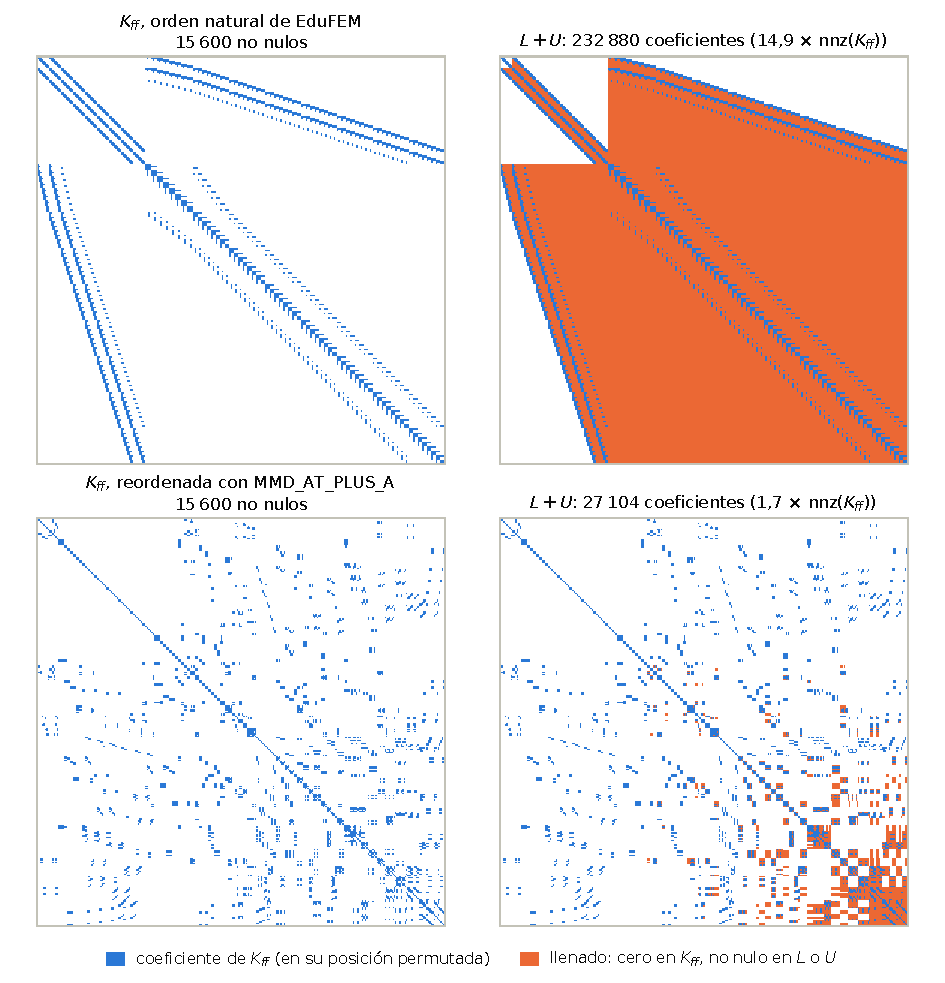
\includegraphics[width=\textwidth]{figuras/llenado_cook.pdf}
  \caption{Patrón de la matriz que SuperLU factoriza y de sus factores, membrana de Cook $8\times8$ Q9 (\cifra{q9:8:n} GDL libres). Arriba: numeración de EduFEM, sin reordenar; los bloques alejados de la diagonal son los nodos intermedios y centrales de los Q9, que la expansión de Q4 a Q9 numera al final. Abajo: la misma matriz reordenada con \ordMMD; la parte densa de $\bm{L}+\bm{U}$ se concentra en el ángulo inferior derecho, donde quedaron los separadores.}
  \label{fig:llenado}
\end{figure}

\begin{figure}[htbp]
  \centering
  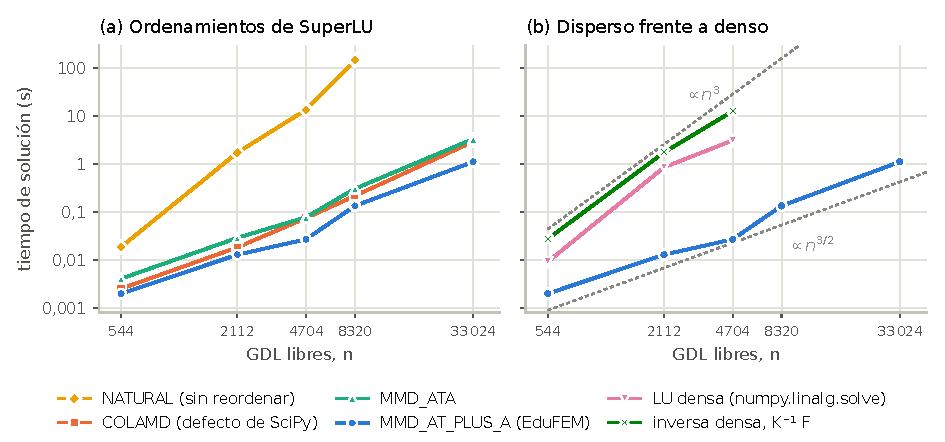
\includegraphics[width=\textwidth]{figuras/tiempos.pdf}
  \caption{Tiempo de solución frente al número de GDL libres (ejes logarítmicos; los valores exactos están en las tablas~\ref{tab:denso} y~\ref{tab:tiempo}). (a)~Los cuatro ordenamientos de SuperLU. (b)~SuperLU con \ordMMD{} frente a los dos caminos densos; las líneas punteadas marcan pendientes de referencia.}
  \label{fig:tiempos}
\end{figure}

\begin{resultado}[title={Qué dicen las mediciones}]
\begin{itemize}[leftmargin=1.2em]
  \item \ordMMD{} produce el menor llenado en todas las mallas: \cifra{q9:64:rel:MMD_AT_PLUS_A} veces $\nnz(\Kff)$ con \cifra{q9:64:n} GDL, contra \cifra{q9:64:rel:COLAMD} de \ordCOLAMD{} y \cifra{q9:64:rel:MMD_ATA} de \ordATA. Con ese tamaño, \ordCOLAMD{} hace \cifra{q9:64:xflops:COLAMD} veces más operaciones y tarda \cifra{q9:64:t:COLAMD}~s frente a \cifra{q9:64:t:MMD_AT_PLUS_A}~s: \cifra{q9:64:x:COLAMD} veces más.
  \item Sin reordenar, el llenado se dispara en Q9: con \cifra{q9:32:n} GDL, $\bm{L}+\bm{U}$ tiene \cifra{q9:32:lu:NATURAL} coeficientes (\cifra{q9:32:rel:NATURAL} veces $\Kff$), la factorización hace \cifra{q9:32:xflops:NATURAL} veces más operaciones que con \ordMMD{} y la solución tarda \cifra{q9:32:t:NATURAL}~s, \cifra{q9:32:x:NATURAL} veces más. La causa es la numeración: la expansión a Q9 agrega los nodos nuevos al final, lejos de sus vecinos.
  \item El llenado con \ordMMD{} crece despacio: al multiplicar $n$ por \cifra{crece:n}, la razón $\nnz(\bm{L}+\bm{U})/\nnz(\Kff)$ pasa de \cifra{q9:8:rel:MMD_AT_PLUS_A} a \cifra{q9:64:rel:MMD_AT_PLUS_A}, coherente con el $O(n\log n)$ de las mallas planas. Las operaciones crecieron \cifra{crece:flops} veces, como $n^{\cifra{expo:flops}}$: algo más que el $n^{3/2}$ de la disección anidada, que el mínimo grado no garantiza, y muchísimo menos que el $n^3$ denso. El tiempo medido creció menos, \cifra{crece:t} veces, porque la velocidad de cálculo sube con el tamaño: de \cifra{q9:8:gflops} a \cifra{q9:64:gflops}~GFLOP/s, a medida que los supernodos crecen y el costo fijo de cada llamada pierde peso.
\end{itemize}
\end{resultado}

Con elementos Q4 y numeración por filas, la numeración natural ya es razonable ---es una numeración de banda---, y la ventaja de \ordMMD{} es menor pero se mantiene (tabla~\ref{tab:q4}). La conclusión práctica es que el ordenamiento independiza al solucionador de la numeración que haya elegido el usuario.

\begin{table}[htbp]
\centering
\caption{Llenado $\nnz(\bm{L}+\bm{U})/\nnz(\Kff)$ con elementos Q4 (membrana de Cook), en mallas con los mismos GDL que las Q9 de la tabla~\ref{tab:llenado}. Última columna: la numeración natural de Q9 con igual $n$, para comparar.}
\label{tab:q4}
\small
\begin{tabular}{rrccccc}
\toprule
$n$ & $\nnz(\Kff)$ & \ordNAT & \ordCOLAMD & \ordATA & \ordMMD & \ordNAT{} en Q9 \\
\midrule
\filas{datos/tabla_q4.tex}
\bottomrule
\end{tabular}
\end{table}

% ══════════════════════════════════════════════════════════════════════════
\section{SuperLU por dentro}\label{sec:superlu}

\subsection{Qué es}

SuperLU es una biblioteca en C para la factorización LU de matrices dispersas generales con pivoteo parcial, desarrollada por Demmel, Eisenstat, Gilbert, Li y Liu~\cite{demmel1999,li2005}. SciPy~\cite{virtanen2020} incluye su versión secuencial compilada dentro de \cod{scipy.sparse.linalg} y la expone con dos funciones, \cod{spsolve} y \cod{splu}. El «\emph{Super}» del nombre viene de los \emph{supernodos} (§\ref{sec:supernodos}).

\subsection{La factorización que calcula}

SuperLU calcula
\begin{equation}\label{eq:superlu}
\boxed{\;\bm{P}_r\,\bm{A}\,\bm{P}_c=\bm{L}\,\bm{U}\;}
\end{equation}
donde $\bm{P}_c$ permuta las columnas según el ordenamiento (§\ref{sec:md}) y $\bm{P}_r$ permuta las filas según el pivoteo. Así es como lo documenta SciPy (\cod{Pr @ A @ Pc = L @ U}). Para resolver $\bm{A}\bm{x}=\bm{b}$:
\begin{equation}
\bm{A}\bm{x}=\bm{b}\iff\underbrace{\bm{P}_r\bm{A}\bm{P}_c}_{\bm{L}\bm{U}}\,\underbrace{\bm{P}_c\T\bm{x}}_{\bm{z}}=\bm{P}_r\bm{b},
\end{equation}
es decir, cuatro pasos: reordenar $\hat{\bm{b}}=\bm{P}_r\bm{b}$; sustituir hacia adelante $\bm{L}\bm{y}=\hat{\bm{b}}$; sustituir hacia atrás $\bm{U}\bm{z}=\bm{y}$; y deshacer el orden, $\bm{x}=\bm{P}_c\bm{z}$. Si el pivoteo elige siempre el coeficiente diagonal, $\bm{P}_r=\bm{P}_c\T$ y la ecuación~\eqref{eq:superlu} es la renumeración simétrica $\bm{P}\mK\bm{P}\T$ de la sección~\ref{sec:llenado}.

\subsection{Las cuatro fases}

\cod{spsolve} llama al controlador simple de SuperLU, \cod{dgssv}, que encadena cuatro fases:
\begin{enumerate}
  \item \textbf{Ordenamiento} (\cod{get_perm_c}): calcula $\bm{P}_c$ según \cod{permc_spec}. Con \ordMMD, arma el patrón de $\bm{A}\T+\bm{A}$ y llama a \cod{GENMMD}.
  \item \textbf{Preordenamiento} (\cod{sp_preorder}): aplica $\bm{P}_c$, calcula el \emph{árbol de eliminación} de las columnas y lo recorre en postorden, que reordena levemente $\bm{P}_c$ sin cambiar el llenado, de modo que las columnas de cada rama y de cada supernodo queden contiguas.
  \item \textbf{Factorización numérica} (\cod{dgstrf}): columna por columna, de izquierda a derecha, agrupando columnas en paneles y supernodos, con pivoteo parcial por umbral. Como el pivoteo puede cambiar la estructura, el cálculo simbólico (qué coeficientes serán no nulos) y el numérico se hacen juntos.
  \item \textbf{Sustituciones} (\cod{dgstrs}): las dos resoluciones triangulares, con las permutaciones.
\end{enumerate}

\subsection{El árbol de eliminación}

El padre de la columna $j$ en el árbol de eliminación es la fila del primer no nulo de $\bm{L}$ debajo de la diagonal:
\begin{equation}
\operatorname{padre}(j)=\min\{\,i>j:\ \ell_{ij}\neq0\,\}.
\end{equation}
La columna $j$ solo puede modificar a sus ancestros, así que dos ramas distintas del árbol no dependen una de otra~\cite{liu1990}. En la estrella (§\ref{sec:estrella}), con el orden B, $\ell_{41},\ell_{42},\ell_{43}\neq0$: las columnas 1, 2 y 3 tienen por padre a la 4, y el árbol es la propia estrella, con tres hojas independientes. Con el orden A, el padre de 1 es 2, el de 2 es 3 y el de 3 es 4: una cadena en la que cada columna espera a la anterior. Los buenos órdenes producen árboles bajos y frondosos; los malos, cadenas.

\subsection{Factorización por columnas, «mirando a la izquierda»}\label{sec:izquierda}

SuperLU calcula la columna $j$ de $\bm{L}$ y $\bm{U}$ usando las columnas ya terminadas, que están a su izquierda. Con $\bm{a}_j$ la columna $j$ de la matriz ya permutada:
\begin{align}
\bm{u}_{1:j-1,\,j}&=\bm{L}_{1:j-1,\,1:j-1}^{-1}\;\bm{a}_{1:j-1,\,j}
  &&\text{(resolución triangular dispersa)}\\
\bm{w}&=\bm{a}_{j:n,\,j}-\bm{L}_{j:n,\,1:j-1}\;\bm{u}_{1:j-1,\,j}
  &&\text{(actualización con las columnas previas)}\\
u_{jj}&=w_p,\qquad \bm{\ell}_{j+1:n,\,j}=\bm{w}_{\text{resto}}/u_{jj}
  &&\text{(pivote $w_p$ elegido por umbral, §\ref{sec:umbral})}
\end{align}
(La «inversa» de $\bm{L}$ en la primera línea es notación: se resuelve por sustitución, ecuación~\eqref{eq:adelante}.) La clave dispersa está en la primera línea: $\bm{u}_{1:j-1,j}$ solo tiene no nulos en las posiciones alcanzables, en el grafo de $\bm{L}$, desde los no nulos de $\bm{a}_j$, y una búsqueda en profundidad las encuentra en un tiempo proporcional a las operaciones útiles~\cite{gilbert1988}. Nunca se recorre un cero.

\subsection{Supernodos}\label{sec:supernodos}

Un \textbf{supernodo} es un grupo de columnas contiguas de $\bm{L}$ con la misma estructura debajo de su bloque diagonal. SuperLU guarda cada supernodo como un bloque denso rectangular, y entonces la actualización con todo el supernodo se convierte en operaciones densas ---una resolución triangular y un producto matriz--vector---, y al procesar varias columnas $j$ a la vez (un panel), en productos matriz--matriz, que aprovechan la memoria caché del procesador mucho mejor que operar coeficiente por coeficiente~\cite{demmel1999}.

En el MEF los supernodos aparecen solos: los dos GDL de un nodo son indistinguibles (§\ref{sec:nodos-gdl}) y forman al menos un supernodo de dos columnas. Medido con \ordMMD{} en la malla de \cifra{q9:64:n} GDL: el tamaño medio de los supernodos fundamentales de $\bm{L}$ es de \cifra{q9:64:sn:media} columnas (unos dos nodos), el \cifra{q9:64:sn:mayor1}\,\% tiene al menos dos columnas y el mayor tiene \cifra{q9:64:sn:max}: es el bloque denso del último separador, el ángulo inferior derecho de la figura~\ref{fig:llenado}.

\subsection{Pivoteo por umbral}\label{sec:umbral}

En la columna $j$, con $\bm{w}$ el vector de candidatos a pivote, SuperLU acepta el coeficiente diagonal si
\begin{equation}
|w_{\text{diag}}|\;\ge\;u\cdot\max_i|w_i|,\qquad u\in[0,1],
\end{equation}
y si no, toma el de mayor módulo. $u=1$ es el pivoteo parcial clásico (la diagonal se acepta solo si es la mayor) y $u=0$ acepta siempre la diagonal si no es nula. \cod{spsolve} no expone este parámetro y usa el valor por defecto de SuperLU, $u=1$; \cod{splu} lo expone como \cod{diag_pivot_thresh}.

Para una $\Kff$ SPD el pivote diagonal es estable (§\ref{sec:pivoteo}), pero con $u=1$ SuperLU puede igualmente intercambiar filas cuando en alguna columna un coeficiente fuera de la diagonal supera al diagonal, algo posible en una SPD: en $\bigl[\begin{smallmatrix}1&2\\2&5\end{smallmatrix}\bigr]$ la primera columna tiene $2>1$. Medido con \cifra{q9:64:n} GDL: $\bm{P}_r$ difiere de $\bm{P}_c\T$ en \cifra{q9:64:piv:MMD_AT_PLUS_A} posiciones (el \cifra{q9:64:pivpct}\,\%), y el llenado es idéntico al que se obtiene forzando la diagonal con $u=0$: \cifra{q9:64:lu:MMD_AT_PLUS_A} coeficientes en ambos casos. Esos intercambios no alteran la estructura que predijo el mínimo grado.

\subsection{\texorpdfstring{\cod{spsolve}}{spsolve} frente a \texorpdfstring{\cod{splu}}{splu}}\label{sec:spsolve-splu}

\begin{itemize}
  \item \cod{spsolve(A, b, permc_spec=...)} ---la que usa EduFEM--- factoriza y resuelve en una sola llamada (\cod{dgssv}) y descarta $\bm{L}$ y $\bm{U}$. Es lo natural con un solo vector de cargas.
  \item \cod{splu(A, permc_spec=...,} \cod{diag_pivot_thresh=...)} factoriza (\cod{dgstrf}) y devuelve un objeto con \cod{L}, \cod{U}, \cod{perm_r}, \cod{perm_c} y un método \cod{solve(b)} que reutiliza los factores. Conviene cuando hay varios vectores de carga.
\end{itemize}
Las dos usan la misma biblioteca y el mismo parámetro \cod{permc_spec} con el mismo significado; la nota al pie de la tesis que menciona la opción \ordMMD{} de \cod{splu} describe, por eso, lo que hace \cod{spsolve}. Un detalle más: \cod{spsolve} usaría UMFPACK en lugar de SuperLU si el paquete \cod{scikits.umfpack} estuviera instalado; en el entorno de EduFEM no lo está, así que el camino es siempre SuperLU.

% ══════════════════════════════════════════════════════════════════════════
\section{El solucionador de EduFEM, pieza por pieza}\label{sec:codigo}

\subsection{El recorrido completo}

La figura~\ref{fig:tuberia} resume lo que ocurre al pulsar «Resolver» (F5). La función pública es \cod{solve_system} de \cod{fem/solver.py}, que recibe el proyecto y devuelve $\bm{u}$, las reacciones y las matrices intermedias.

\begin{figure}[htbp]
\centering
\newcommand{\npy}{\textcolor{serie1!70!black}{\textbf{NumPy}}}
\newcommand{\spy}{\textcolor{serie3!55!black}{\textbf{SciPy}}}
\newcommand{\slu}{\textcolor{serie2!75!black}{\textbf{SuperLU (C)}}}
\newcommand{\pasotub}[3]{\parbox[t]{9.6cm}{\raggedright #1}\hfill\parbox[t]{4.7cm}{\raggedleft\footnotesize #2\\ #3}}
\begin{tikzpicture}[
  caja/.style={draw=#1!70!black,fill=#1!8,rounded corners=2pt,line width=0.5pt,text width=14.4cm,inner sep=3.5pt,font=\small,align=left},
  flecha/.style={-{Stealth[length=1.8mm]},line width=0.6pt,draw=tinta2},
  node distance=1.8mm]
  \node[caja=serie1] (p1) {\pasotub{\textbf{1. Rigideces elementales}, de todos los elementos a la vez:\\ $\bm{k}_e=\sum_g\bm{B}_g\T\bm{D}\bm{B}_g\,t\,|J_g|\,w_g$}{\cod{stiffness_batch}}{\npy}};
  \node[caja=serie1,below=of p1] (p2) {\pasotub{\textbf{2. Tripletes} $\bigl(i,\,j,\,(\bm{k}_e)_{ab}\bigr)$ de todos los elementos}{\cod{np.repeat}, \cod{np.tile}, \cod{ravel}}{\npy}};
  \node[caja=serie3,below=of p2] (p3) {\pasotub{\textbf{3. $\mK$ en CSR}: COO $\to$ CSR sumando los repetidos, que es el ensamblaje}{\cod{coo_matrix(...).tocsr()}}{\spy}};
  \node[caja=serie3,below=of p3] (p4) {\pasotub{\textbf{4. Sistema reducido}: máscara de GDL libres, $\Kff=\mK[f,f]$ y $\bm{F}_f-\mK_{fr}\bm{u}_r$}{\cod{np.where}; indexado disperso}{\npy{} + \spy}};
  \node[caja=serie3,below=of p4] (p5) {\pasotub{\textbf{5. $\Kff$ en CSC}, el formato por columnas de SuperLU}{\cod{K_red.tocsc()}}{\spy}};
  \node[caja=serie2,below=of p5] (p6) {\pasotub{\textbf{6. Ordenar, factorizar y sustituir}:\\
    6a.\ mínimo grado múltiple sobre el patrón de $\Kff\T+\Kff$ $\to$ $\bm{P}_c$\\
    6b.\ árbol de eliminación y postorden\\
    6c.\ $\bm{P}_r\Kff\bm{P}_c=\bm{L}\bm{U}$, por columnas, con supernodos y pivoteo por umbral\\
    6d.\ $\bm{L}\bm{y}=\bm{P}_r\bm{F}_f$,\ \ $\bm{U}\bm{z}=\bm{y}$,\ \ $\bm{u}_f=\bm{P}_c\bm{z}$}{\cod{spsolve(K_red.tocsc(), F_red,}\\ \cod{permc_spec="MMD_AT_PLUS_A")}}{\slu}};
  \node[caja=serie1,below=of p6] (p7) {\pasotub{\textbf{7. Control}: si hay \cod{NaN} o \cod{Inf}, $\Kff$ era singular (mecanismo) y se avisa}{\cod{np.isfinite}}{\npy}};
  \node[caja=serie1,below=of p7] (p8) {\pasotub{\textbf{8. Vector completo} $\bm{u}$: los libres calculados y los restringidos prescritos}{indexado}{\npy}};
  \node[caja=serie3,below=of p8] (p9) {\pasotub{\textbf{9. Reacciones} $\bm{R}_r=\mK[r,:]\,\bm{u}-\bm{F}_r$, solo en las filas restringidas}{producto disperso}{\spy}};
  \foreach \a/\b in {p1/p2,p2/p3,p3/p4,p4/p5,p5/p6,p6/p7,p7/p8,p8/p9}
    \draw[flecha] (\a.south) -- (\b.north);
\end{tikzpicture}
\caption{El camino de \cod{solve_system}. Azul: NumPy (arreglos densos); verde agua: \cod{scipy.sparse} (matrices dispersas); naranja: SuperLU, la biblioteca en C que SciPy incluye.}
\label{fig:tuberia}
\end{figure}

\subsection{El código}

El ordenamiento se fija en una sola constante, con la medición que lo justifica en el comentario:

\begin{lstlisting}[style=py,firstnumber=467,caption={\cod{config/settings.py}.}]
# Ordenamiento de columnas de SuperLU (`permc_spec` de scipy.sparse.linalg.spsolve).
# K es simetrica y definida positiva: "MMD_AT_PLUS_A" (minimo grado sobre
# A^T + A) reduce el llenado de la factorizacion LU frente al default
# "COLAMD", pensado para matrices no simetricas. Medido en la membrana de Cook
# (spsolve sobre K_red ya en CSC): 2178 GDL 14,3 -> 9,1 ms (1,6x);
# 8450 GDL 128 -> 61 ms (2,1x); 33 282 GDL 888 -> 421 ms (2,1x). |du| ~ 3e-11.
SOLVER_PERMC_SPEC = "MMD_AT_PLUS_A"
\end{lstlisting}

El sistema reducido se arma con una máscara booleana. \cod{K[free_arr, :]} selecciona filas (rápido en CSR) y \cod{[:, free_arr]}, columnas; el resultado es $\Kff$, ecuación~\eqref{eq:reducido}:

\begin{lstlisting}[style=py,firstnumber=44,caption={\cod{fem/solver.py}, \cod{apply_boundary_conditions} (sin el docstring).}]
    rest_arr = np.asarray(restrained_dofs, dtype=np.intp)
    mask = np.ones(n_dof, dtype=bool)
    if rest_arr.size > 0:
        mask[rest_arr] = False
    free_arr = np.where(mask)[0]
    free_dofs = free_arr.tolist()  # API legacy retorna list

    # Indexado por filas luego columnas — eficiente en CSR y correcto en denso.
    K_red = K[free_arr, :][:, free_arr]
    # spsolve requiere CSR o CSC; .tocsr() es no-op si ya es CSR.
    try:
        K_red = K_red.tocsr()
    except AttributeError:
        pass  # K denso (tests de backward-compat): se pasa directo a spsolve

    F_red = F[free_arr].copy()

    if u_prescribed is not None and rest_arr.size > 0:
        u_r = u_prescribed[rest_arr]
        if np.any(u_r != 0.0):
            K_fr = K[free_arr, :][:, rest_arr]
            F_red -= np.asarray(K_fr @ u_r).ravel()
\end{lstlisting}

Y la solución propiamente dicha es una línea: todo lo de las secciones~\ref{sec:lu} a~\ref{sec:superlu} ocurre dentro de \cod{spsolve}.

\begin{lstlisting}[style=py,firstnumber=80,caption={\cod{fem/solver.py}, \cod{_solve_reduced} (sin el docstring).}]
    from config.settings import SOLVER_PERMC_SPEC

    if not hasattr(K_red, "tocsc"):
        return spsolve(K_red, F_red)

    return spsolve(K_red.tocsc(), F_red, permc_spec=SOLVER_PERMC_SPEC)
\end{lstlisting}

La rama con \cod{hasattr} solo existe para pruebas antiguas que pasan una matriz densa. Después, \cod{solve_system} controla el resultado, completa $\bm{u}$ y calcula las reacciones:

\begin{lstlisting}[style=py,firstnumber=133,caption={\cod{fem/solver.py}, \cod{solve_system}, pasos 5 a 7.}]
    u_free = _solve_reduced(K_red, F_red)
    if np.any(~np.isfinite(u_free)):
        raise ValueError(
            "El solver produjo valores NaN o Inf. Verifica que K no sea "
            "singular: modelo mal restringido, elemento degenerado o E/ν fuera "
            "de rango pueden causar este problema."
        )

    # 6. Reconstruir vector completo de desplazamientos.
    #    En DOFs libres: valor calculado. En DOFs restringidos: valor prescrito.
    # Fancy indexing vectorizado (no loop Python).
    u = np.zeros(project.total_dof)
    free_arr = np.asarray(free_dofs, dtype=np.intp)
    u[free_arr] = u_free
    if u_prescribed is not None and len(restrained_dofs) > 0:
        rest_arr = np.asarray(restrained_dofs, dtype=np.intp)
        u[rest_arr] = u_prescribed[rest_arr]

    # 7. Calcular reacciones: R = K · u - F, SOLO en los GDL restringidos.
    #    En los GDL libres R es ~0 (residuo numerico ~1e-12); ponerlo en 0
    #    exacto evita la multiplicacion densa K @ u completa (solo se evaluan
    #    las filas restringidas) y deja R limpio para lectura/reporte.
    reactions = np.zeros(project.total_dof)
    if len(restrained_dofs) > 0:
        rest = np.asarray(restrained_dofs, dtype=np.intp)
        reactions[rest] = np.asarray(K[rest, :] @ u).ravel() - F[rest]
\end{lstlisting}

La última línea es la ecuación~\eqref{eq:reacciones} escrita con la matriz completa: $\mK[r,:]\,\bm{u}-\bm{F}_r=\mK_{rf}\bm{u}_f+\mK_{rr}\bm{u}_r-\bm{F}_r$.

\subsection{Qué hace NumPy y qué hace SciPy}

\begin{center}
\small
\begin{tabularx}{\textwidth}{>{\raggedright\arraybackslash}p{3.5cm}>{\raggedright\arraybackslash}X>{\raggedright\arraybackslash}p{3.9cm}}
\toprule
Biblioteca & Qué hace en el solucionador & Funciones \\
\midrule
NumPy & Arreglos densos: el lote de $\bm{k}_e$, los tripletes, la máscara de GDL libres, los vectores $\bm{F}$, $\bm{u}$ y $\bm{R}$, el control de \cod{NaN}. & \cod{einsum}, \cod{matmul}, \cod{repeat}, \cod{tile}, \cod{where}, \cod{isfinite} \\
\cod{scipy.sparse} & Matrices dispersas: COO, CSR y CSC, la suma de repetidos, la extracción de $\Kff$ y $\mK_{fr}$, los productos matriz--vector. & \cod{coo_matrix}, \cod{tocsr}, \cod{tocsc}, indexado, \cod{@} \\
SuperLU, dentro de \cod{scipy.sparse.linalg} & Ordenamiento, árbol de eliminación, factorización con supernodos y pivoteo, sustituciones. & \cod{spsolve} \\
\bottomrule
\end{tabularx}
\end{center}

NumPy~\cite{harris2020} tiene su propio solucionador, \cod{numpy.linalg.solve}, pero es denso: también factoriza ---llama a la rutina \cod{gesv} de LAPACK, una LU con pivoteo parcial---, pero sobre los $n^2$ coeficientes. Es la columna «LU densa» de la tabla~\ref{tab:denso}. \cod{numpy.linalg.inv}, por su parte, factoriza y después resuelve $n$ sistemas, uno por cada columna de la identidad.

\subsection{Traza de una resolución real}

Todo lo anterior, con los números de una corrida del motor sobre la membrana de Cook de $8\times8$ elementos Q9:

\begin{paso}[title={Membrana de Cook, $8\times8$ Q9}]
\begin{enumerate}[leftmargin=1.4em]
  \item \textbf{Malla}: \cifra{q9:8:nodos} nodos, \cifra{q9:8:elementos} elementos, \cifra{q9:8:gdl} GDL.
  \item \textbf{Lote}: \cifra{q9:8:elementos} matrices $\bm{k}_e$ de $18\times18$ $\to$ \cifra{q9:8:tripletes} tripletes.
  \item \textbf{\cod{coo_matrix(...).tocsr()}}: suma \cifra{q9:8:duplicados} repetidos $\to$ $\mK$ con \cifra{q9:8:nnzK} no nulos, el \cifra{q9:8:densK}\,\% de $\cifra{q9:8:gdl}^2$.
  \item \textbf{Restricciones}: \cifra{q9:8:restr} GDL restringidos (los nodos del borde empotrado) $\to$ $n=\cifra{q9:8:n}$ libres; $\Kff$ con \cifra{q9:8:nnzKr} no nulos.
  \item \textbf{\cod{spsolve(K_red.tocsc(), F_red, permc_spec="MMD_AT_PLUS_A")}}: $\bm{L}+\bm{U}$ con \cifra{q9:8:figLU:MMD} coeficientes, \cifra{q9:8:rel:MMD_AT_PLUS_A} veces $\nnz(\Kff)$ (sin reordenar habrían sido \cifra{q9:8:figLU:NATURAL}); tiempo: \cifra{q9:8:ms:MMD_AT_PLUS_A}~ms.
  \item \textbf{Control}: residuo $\|\Kff\bm{u}_f-\bm{F}_f\|/\|\bm{F}_f\|=\cifra{traza:resid}$. Desplazamiento vertical en el centro del lado cargado, $(48,52)$: $u_y=\cifra{traza:uyC}$, el mismo valor que reporta la verificación de la tesis para esta malla (\cod{docs/vyv/datos/cook.csv}; valor de referencia publicado, \cifra{traza:uyRef}).
  \item \textbf{Reacciones}: $\sum R_y=\cifra{traza:sumRy}$ frente a $\sum F_y=\cifra{traza:sumFy}$; $|\sum R_x|=\cifra{traza:sumRx}$. El equilibrio global se cumple.
\end{enumerate}
\end{paso}

\subsection{Cómo se comprueba que el solucionador está bien}

\begin{itemize}
  \item \textbf{Residuo}: $\|\Kff\bm{u}_f-\bm{F}_f\|/\|\bm{F}_f\|$ del orden de $10^{-12}$ en todas las mallas (tabla~\ref{tab:denso}).
  \item \textbf{Equilibrio}: la suma de reacciones equilibra la suma de cargas, como en la traza.
  \item \textbf{Regresión}: \cod{tests/test_solver_regression.py} compara el motor por lotes con la versión legible elemento a elemento (error relativo $\le10^{-9}$), y \cod{tests/test_fem.py} verifica Q4, Q9 y las cargas superficiales.
  \item \textbf{Ordenamiento}: \cod{tests/bench_timing.py} mide \ordCOLAMD{} frente a \ordMMD{} sobre el mismo sistema; cambiar el ordenamiento cambia $\bm{u}$ solo en el redondeo (del orden de $10^{-11}$, según el comentario de \cod{config/settings.py}).
  \item \textbf{Verificación y validación}: la membrana de Cook, la viga de Timoshenko y las soluciones manufacturadas de la tesis ejercitan el mismo camino.
\end{itemize}

% ══════════════════════════════════════════════════════════════════════════
\section{Preguntas que pueden aparecer en la defensa}\label{sec:defensa}

\begin{description}[style=nextline,leftmargin=1em,labelindent=0pt,itemsep=6pt]
  \item[¿EduFEM invierte la matriz de rigidez?]
  No. Factoriza $\Kff=\bm{L}\bm{U}$ con SuperLU y obtiene $\bm{u}_f$ por sustitución hacia adelante y hacia atrás. La inversa sería llena (medido: el \cifra{q9:24:densInv}\,\% de coeficientes no nulos), costaría tres veces más operaciones incluso en denso y con \cifra{q9:64:n} GDL ocuparía \cifra{q9:64:gbInv}~GB.

  \item[Entonces, ¿qué significa $\bm{u}=\bm{K}^{-1}\bm{F}$ en la tesis?]
  Es la notación de la solución única, que existe porque $\Kff$ es SPD. El algoritmo que la calcula es factorizar y sustituir.

  \item[¿Qué es la factorización LU?]
  La eliminación de Gauss con los multiplicadores guardados: $\bm{A}=\bm{L}\bm{U}$, donde $\bm{L}$ (triangular inferior) reúne los multiplicadores y $\bm{U}$ (triangular superior) es lo que queda al eliminar. Después, $\bm{L}\bm{y}=\bm{F}$ y $\bm{U}\bm{u}=\bm{y}$.

  \item[Si $\bm{K}$ es SPD, ¿por qué no Cholesky?]
  Cholesky haría la mitad de operaciones y de memoria, pero SciPy no la trae en formato disperso: habría que agregar \cod{scikit-sparse} (CHOLMOD), una dependencia binaria más para el instalador. Con \ordMMD{} y pivotes diagonales, la LU tiene la misma estructura que Cholesky ($\bm{U}=\bm{D}\bm{L}\T$): la diferencia es un factor cercano a 2, no un cambio de orden. Queda como recomendación de la tesis.

  \item[¿Qué es SuperLU?]
  Una biblioteca en C de factorización LU dispersa con pivoteo parcial (Demmel, Gilbert, Li y otros), incluida en SciPy. «Super» por los supernodos: grupos de columnas con la misma estructura que se procesan como bloques densos, lo que la hace rápida.

  \item[¿Qué es el llenado y por qué importa?]
  Son los coeficientes nulos en $\mK$ que dejan de serlo en $\bm{L}$ o $\bm{U}$. Cuestan memoria y tiempo, y dependen del orden en que se eliminan las incógnitas. Con \cifra{q9:32:n} GDL: sin reordenar, \cifra{q9:32:lu:NATURAL} coeficientes y \cifra{q9:32:t:NATURAL}~s; con mínimo grado, \cifra{q9:32:lu:MMD_AT_PLUS_A} y \cifra{q9:32:t:MMD_AT_PLUS_A}~s.

  \item[¿Qué hace el ordenamiento de mínimo grado?]
  Elige, en cada paso, eliminar la incógnita con menos conexiones, porque eliminar una incógnita conecta entre sí a todos sus vecinos: la de menor grado es la que menos llenado crea en ese paso. Es una heurística; encontrar el orden óptimo es un problema NP-completo.

  \item[¿Por qué $\bm{K}^{\top}+\bm{K}$ si $\bm{K}$ ya es simétrica?]
  Porque SuperLU está hecho para matrices generales y el mínimo grado necesita un grafo no dirigido: $\bm{A}\T+\bm{A}$ simetriza el patrón. Para $\mK$, $\mK\T+\mK=2\mK$ tiene el mismo patrón, así que es el mínimo grado sobre el grafo de la propia malla.

  \item[¿Por qué no el ordenamiento por defecto de SciPy (COLAMD)?]
  \ordCOLAMD{} ordena pensando en $\bm{A}\T\bm{A}$, lo que protege contra cualquier pivoteo en matrices no simétricas. Para $\mK$, $\bm{A}\T\bm{A}=\mK^2$ une GDL a dos elementos de distancia, un modelo más grueso: con \cifra{q9:64:n} GDL da más llenado (\cifra{q9:64:rel:COLAMD} contra \cifra{q9:64:rel:MMD_AT_PLUS_A} veces $\nnz(\Kff)$), hace \cifra{q9:64:xflops:COLAMD} veces más operaciones y tarda \cifra{q9:64:x:COLAMD} veces más.

  \item[¿El reordenamiento cambia la solución?]
  No: resuelve el mismo sistema con las ecuaciones en otro orden, $(\bm{P}\mK\bm{P}\T)(\bm{P}\bm{u})=\bm{P}\bm{F}$. Solo cambia el redondeo, en el orden de $10^{-11}$ relativo.

  \item[¿Hay pivoteo? ¿Es estable?]
  SuperLU usa pivoteo parcial por umbral ($u=1$ en \cod{spsolve}). En $\Kff$ SPD elige casi siempre la diagonal (difiere en \cifra{q9:64:piv:MMD_AT_PLUS_A} de \cifra{q9:64:n} posiciones) sin cambiar el llenado. Una matriz SPD es estable incluso sin pivoteo: sus pivotes son positivos y los coeficientes no crecen.

  \item[¿Qué es COO y por qué después CSR y CSC?]
  COO es la lista de tripletes (fila, columna, valor); admite repetidos, que se suman: eso es el ensamblaje. CSR agrupa por filas, lo que sirve para extraer $\Kff$ y calcular reacciones; CSC agrupa por columnas, que es como trabaja SuperLU.

  \item[¿Qué hace NumPy y qué hace SciPy?]
  NumPy maneja los arreglos densos: el lote de $\bm{k}_e$, los tripletes, las máscaras y los vectores. SciPy maneja las matrices dispersas y el solucionador; SuperLU es código C compilado dentro de SciPy.

  \item[¿Por qué un solucionador directo y no uno iterativo (gradiente conjugado)?]
  En los tamaños de uso formativo el directo es robusto ---no depende del condicionamiento ni de un precondicionador--- y rápido: \cifra{q9:64:t:MMD_AT_PLUS_A}~s con \cifra{q9:64:n} GDL en un portátil de 2012. El iterativo precondicionado queda entre las recomendaciones para mallas muy grandes.

  \item[¿Qué pasa si el modelo está mal restringido?]
  $\Kff$ es singular: aparece un pivote nulo, SuperLU lo informa, SciPy devuelve \cod{NaN} y EduFEM detiene el cálculo con un mensaje que apunta a un modelo mal restringido o a un elemento degenerado. El validador de salud del modelo avisa antes de llegar a resolver.

  \item[¿Cómo sé que la solución es correcta?]
  Residuo relativo del orden de $10^{-12}$, equilibrio de reacciones, el test de regresión contra la versión legible del motor y la verificación y validación de la tesis (Cook, Timoshenko, soluciones manufacturadas).
\end{description}

% ══════════════════════════════════════════════════════════════════════════
\appendix
\section{Conteo de operaciones}\label{ap:flops}

Se cuenta una suma, una resta, un producto o una división como una operación (\emph{flop}).

\textbf{Factorización LU.} En el paso $k$ hay $n-k$ multiplicadores (una división cada uno) y $(n-k)^2$ actualizaciones $a_{ij}-\ell_{ik}a_{kj}$ (un producto y una resta cada una):
\[
\sum_{k=1}^{n-1}\Bigl[(n-k)+2(n-k)^2\Bigr]=\sum_{m=1}^{n-1}\bigl(m+2m^2\bigr)\approx\frac23n^3 .
\]

\textbf{Sustituciones.} La fila $i$ de la ecuación~\eqref{eq:adelante} hace $i-1$ productos y $i-1$ restas: $\sum_i2(i-1)\approx n^2$. La sustitución hacia atrás cuesta lo mismo. Total: $2n^2$.

\textbf{Inversa.} Una vez factorizada la matriz, la columna $j$ de $\bm{A}^{-1}$ resuelve $\bm{L}\bm{U}\bm{x}=\bm{e}_j$. En la sustitución hacia adelante, las primeras $j-1$ componentes de $\bm{y}$ son nulas, así que cuesta $\approx(n-j)^2$; la sustitución hacia atrás cuesta $n^2$ completa. Sumando sobre las $n$ columnas:
\[
\frac23n^3+\sum_{j=1}^{n}(n-j)^2+n\cdot n^2\approx\frac23n^3+\frac13n^3+n^3=2n^3 .
\]

\textbf{Caso disperso.} Si la columna $j$ de $\bm{L}$ tiene $c_j$ no nulos debajo de la diagonal y la fila $j$ de $\bm{U}$ tiene $r_j$ a la derecha de la diagonal, el paso $j$ hace $c_j$ divisiones y $c_j\,r_j$ actualizaciones:
\[
\text{operaciones}=\sum_{j=1}^{n}\bigl(c_j+2\,c_j\,r_j\bigr),
\]
que con patrón simétrico ($r_j=c_j$) es $\sum_j(c_j+2c_j^2)$. Es la cuenta de la tabla~\ref{tab:llenado}, hecha sobre los factores que devuelve SuperLU. El llenado entra \emph{al cuadrado}: por eso reducirlo tiene un efecto tan grande sobre el tiempo. En el caso denso, $c_j=r_j=n-j$ y se recupera el $\tf23n^3$ de arriba.

\section{Cómo reproducir las cifras}\label{ap:reproducir}

Desde la raíz del repositorio, con el entorno del proyecto:
\begin{lstlisting}[style=py,numbers=none]
python docs/teoria/solucionador/generar_datos.py            # todo (unos 5 minutos)
python docs/teoria/solucionador/generar_datos.py --rapido   # sin los casos de mas de 10 s
cd docs/teoria/solucionador
pdflatex solucionador_disperso.tex                         # dos veces, por las referencias
\end{lstlisting}
El guion escribe \cod{datos/cifras.tex} (las cifras del texto), las filas de tabla \cod{datos/tabla_*.tex}, las mediciones en bruto \cod{datos/mediciones.json} y las figuras de \cod{figuras/}. Antes de medir, verifica en aritmética exacta los ejemplos 1 a 4; si alguno dejara de cumplirse, se detiene sin escribir nada.

% ══════════════════════════════════════════════════════════════════════════
\begin{thebibliography}{99}\small
\bibitem{golub2013} Golub GH, Van Loan CF. Matrix computations. 4.ª ed. Baltimore: Johns Hopkins University Press; 2013.
\bibitem{trefethen1997} Trefethen LN, Bau D. Numerical linear algebra. Philadelphia: SIAM; 1997.
\bibitem{higham2002} Higham NJ. Accuracy and stability of numerical algorithms. 2.ª ed. Philadelphia: SIAM; 2002.
\bibitem{davis2006} Davis TA. Direct methods for sparse linear systems. Philadelphia: SIAM; 2006.
\bibitem{davis2016} Davis TA, Rajamanickam S, Sid-Lakhdar WM. A survey of direct methods for sparse linear systems. Acta Numer. 2016;25:383-566.
\bibitem{george1981} George A, Liu JWH. Computer solution of large sparse positive definite systems. Englewood Cliffs: Prentice-Hall; 1981.
\bibitem{parter1961} Parter S. The use of linear graphs in Gauss elimination. SIAM Rev. 1961;3(2):119-30.
\bibitem{rose1972} Rose DJ. A graph-theoretic study of the numerical solution of sparse positive definite systems of linear equations. En: Read RC, editor. Graph theory and computing. New York: Academic Press; 1972. p. 183-217.
\bibitem{markowitz1957} Markowitz HM. The elimination form of the inverse and its application to linear programming. Manage Sci. 1957;3(3):255-69.
\bibitem{tinney1967} Tinney WF, Walker JW. Direct solutions of sparse network equations by optimally ordered triangular factorization. Proc IEEE. 1967;55(11):1801-9.
\bibitem{george1973} George A. Nested dissection of a regular finite element mesh. SIAM J Numer Anal. 1973;10(2):345-63.
\bibitem{yannakakis1981} Yannakakis M. Computing the minimum fill-in is NP-complete. SIAM J Algebraic Discrete Methods. 1981;2(1):77-9.
\bibitem{liu1985} Liu JWH. Modification of the minimum-degree algorithm by multiple elimination. ACM Trans Math Softw. 1985;11(2):141-53.
\bibitem{george1989} George A, Liu JWH. The evolution of the minimum degree ordering algorithm. SIAM Rev. 1989;31(1):1-19.
\bibitem{george1987} George A, Ng E. Symbolic factorization for sparse Gaussian elimination with partial pivoting. SIAM J Sci Stat Comput. 1987;8(6):877-98.
\bibitem{davis2004colamd} Davis TA, Gilbert JR, Larimore SI, Ng EG. A column approximate minimum degree ordering algorithm. ACM Trans Math Softw. 2004;30(3):353-76.
\bibitem{liu1990} Liu JWH. The role of elimination trees in sparse factorization. SIAM J Matrix Anal Appl. 1990;11(1):134-72.
\bibitem{gilbert1988} Gilbert JR, Peierls T. Sparse partial pivoting in time proportional to arithmetic operations. SIAM J Sci Stat Comput. 1988;9(5):862-74.
\bibitem{demmel1999} Demmel JW, Eisenstat SC, Gilbert JR, Li XS, Liu JWH. A supernodal approach to sparse partial pivoting. SIAM J Matrix Anal Appl. 1999;20(3):720-55.
\bibitem{li2005} Li XS. An overview of SuperLU: algorithms, implementation, and user interface. ACM Trans Math Softw. 2005;31(3):302-25.
\bibitem{virtanen2020} Virtanen P, Gommers R, Oliphant TE, Haberland M, Reddy T, Cournapeau D, et al. SciPy 1.0: fundamental algorithms for scientific computing in Python. Nat Methods. 2020;17(3):261-72.
\bibitem{harris2020} Harris CR, Millman KJ, van der Walt SJ, Gommers R, Virtanen P, Cournapeau D, et al. Array programming with NumPy. Nature. 2020;585(7825):357-62.
\bibitem{bathe2014} Bathe KJ. Finite element procedures. 2.ª ed. Watertown (MA): K.J. Bathe; 2014.
\end{thebibliography}

\end{document}
